\chapter{Improved Prediction Models for PALs} % Main chapter title
\label{chap:predict_model} % Change X to a consecutive number; for referencing this chapter elsewhere, use \ref{ChapterX}
\blfootnote{The work presented in this chapter have been published in \cite{Zhong2020SphericalExpansionAudio, Zhong2020SphericalExpansionCalculating, Zhong2021FieldWesterveltFar} and submitted to The Journal of the Acoustical Society of America \cite{Zhong2021CylindricalExpansionAudio}.}

\noindent The prediction models for PALs are very important for PAL applications.
As described in Chap.~\ref{chap:sound_field}, the audio sound field is calculated based on the ultrasound field.
Therefore, the ultrasound is required to obtain first, which can be modelled as a radiation from a baffled piston source.
A SWE for the radiation from a circular piston source is proposed in Sec.~\ref{Section41}, which aims to simplify the two-fold Rayleigh integral.
The SWE is then extended to calculate the radiation from a circular PAL as presented in Sec.~\ref{sec:swe_pal}.
For a rectangular PAL, a CWE is proposed in Sec.~\ref{sec:cwe_pal}, and is used to analyze the radiation from a steerable PAL.

\section{Spherical wave expansion (SWE) for a circular source}
\label{Section41}

The sound radiated by a baffled circular piston can be obtained using Rayleigh integral given by Eq.~(\ref{eq:rayleigh}), which is unsolvable in most cases \cite{Mast2005SimplifiedExpansionsRadiation}. 
The direct numerical integration of Rayleigh integral can be used to obtain the result while the calculation time and required memory size increase significantly with frequency \cite{Zemanek1971BeamBehaviorNearfield}.
The reason accounts for the poor convergency is that the Green's function given by Eq.~(\ref{eq:green_function_free_field}) in the integrand is highly oscillatory.
An efficient but rigorous calculation method currently available is decomposing the integral into a series of spherical harmonics where the angular and radial components are related to Legendre and spherical Bessel functions, respectively \cite{Mast2005SimplifiedExpansionsRadiation, Poletti2018SphericalExpansionsSound}. 
The expression of the series is different in different regions, resulting in paraxial, interior, and exterior expansions. 
The existing methods work fine for the paraxial and interior expansions, but the calculation of the exterior expansion is rather time-consuming at middle and high frequencies which will be focused on in this section. 

The paraxial expansion is used when the distance between the field point and the radiation axis is less than the transducer radius. 
In this expansion, each term of the series is obtained with a finite step of recurrences \cite{Mast2005SimplifiedExpansionsRadiation}.
It converges rapidly, but the coordinates of the field point and the transducer radius are coupled in the argument of special functions. 
Although the paraxial region covers the major energy of a sound beam at high frequencies, it is sometimes necessary to calculate the sound pressure in other regions. For example, the ultrasound outside the paraxial region needs to be taken into consideration, otherwise the prediction of audio sounds generated by nonlinear interactions of intensive ultrasounds would be inaccurate \cite{Cervenka2013NonparaxialModelParametric, Zhong2020SphericalExpansionAudio}.

The interior expansion is valid when the distance between the field point and the transducer center is less than the transducer radius. 
Although the interior expansion converges slowly, the field coordinates are uncoupled in the argument of special functions which means the radial and angular components can be calculated separately for a large number of field points \cite{Mast2005SimplifiedExpansionsRadiation, Poletti2018SphericalExpansionsSound}.
To improve the convergence performance, a feasible technique is estimating the values of truncated terms of the series \cite{Poletti2018SphericalExpansionsSound}.
The interior expansion is not widely used because this region is small and it is also covered by the paraxial region. 

For the field point in the exterior region where the distance between the point and the transducer center is larger than transducer radius, the exterior expansion needs to be used. 
The widely used expression of the exterior expansion is related to the generalized hypergeometric function (GHF).
Although it converges rapidly at low frequencies, its convergence performance is poor at middle and high frequencies because the GHF is an alternating series, the calculation involves subtractions between large numbers resulting in loss of significant figures, and the number of summation terms increases rapidly as the frequency increases. 
Therefore, the extended precision of float numbers in computers or other special techniques have to be used, resulting in an increase of computation complexity \cite{Perger1993NumericalEvaluatorGeneralized, Pearson2009ComputationHypergeometricFunctions}.
Besides, the GHF is difficult to analyze if further operations on the solution are required, such as integrals \cite{Cervenka2013NonparaxialModelParametric, Carley2006SeriesExpansionSound} and derivatives \cite{Carley2010SeriesExpansionSound} with respect to the coordinates and the transducer radius.

In this section, the interior and exterior expansions for Rayleigh integral is given in an easier way.
The integral over spherical Bessel functions is simplified rigorously into a closed-form based on the recurrence method. 
Compared to the existing GHF method, Gauss-Legendre quadrature, and Bessel expansion method, the proposed expression is accurate and computationally efficient in the whole frequency range. 
It can also be extended to other scenarios such as a baffled piston, an unbaffled resilient disk with axisymmetric velocity and pressure profiles, and some baffled rotating sources where the velocity profile is asymmetric.

\subsection{Theory}
% describe the model
The model to be investigated in shown in Fig.~\ref{fig:swe_piston_sketch}.
In this section, we assumed an axisymmetric velocity profile on the transducer surface, i.e., $ u(\rho\subt{s},k)$.

\begin{figure}[!htb]
    \centering
    % 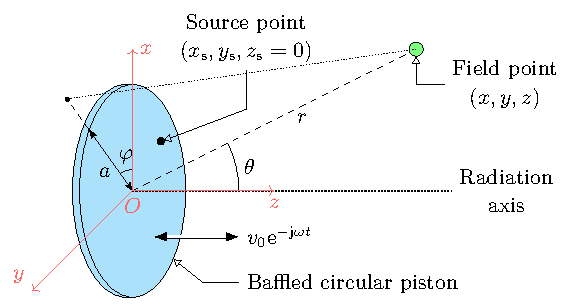
\includegraphics[width = 0.6\textwidth]{E:/Research/PistonComp2001/fig/Piston_Sketch/Piston_Sketch_200923.pdf}
    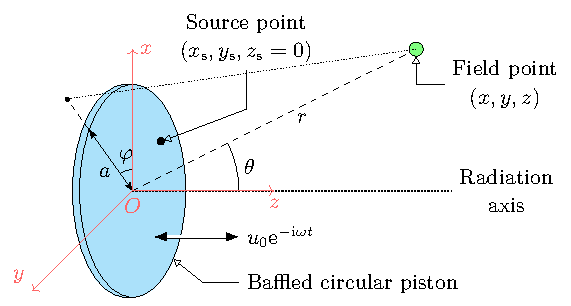
\includegraphics[width = 0.6\textwidth]{fig/Piston_Sketch_200923_v2.pdf}
    \caption{\revA{Sketch of the radiation from a baffled circular rigid piston source.}}
    \label{fig:swe_piston_sketch}
\end{figure}

The sound field generated by the source can be calculated by the Rayleigh integral given by Eq.~(\ref{eq:rayleigh}).
The Green's function in a free field used in Eq.~(\ref{eq:rayleigh}) is given by Eq.~(\ref{eq:green_function_free_field}).
It can be expanded under the spherical coordinates as the summation of spherical harmonic terms \cite{Zhong2020SphericalExpansionAudio}
\begin{equation}
    g(\vb{r}_1,\vb{r}_2, k)
    = 
    \frac{\rmi k }{4\uppi}
    \sum_{n =0}^{\infty} 
    \sum_{m=-n}^n 
    (2n +1)
    \frac{(n-m)!}{(n+m)!}
    \rmj_n (kr_<)
    \rmh_n(kr_>)
    P_n^m(\cos\theta_1)
    P_n^m(\cos\theta_2) \rme^{\rmi m (\varphi_1-\varphi_2)}
    \label{eq:swe_green_expansion}
\end{equation}
where $r_< = \min(r_1,r_2)$, $r_> = \max(r_1,r_2)$, $j_n(\cdot)$ is the spherical Bessel function of order $n$, $h_n(\cdot)$ is the spherical Hankel function of the first kind of order $n$, $P_n^m(\cdot)$ is the associated Legendre function of order $n$ and degree $m$, and $!$ represents the factorial.

From the geometric relation, it is clear that $\theta\subt{s} = \uppi/2$ since $z\subt{s} = 0$.
The substitution of Eq.~(\ref{eq:swe_green_expansion}) into Rayleigh integral given by Eq.~(\ref{eq:rayleigh}) and the utilization of the relation $r\subt{s} = \rho\subt{s}$, yields
\begin{dmath}
    \Phi(\vb{r},k)
  =
  \frac{1}{\rmi k}
  \sum_{n=0}^\infty 
  \sum_{m=-n}^n
  (2n+1)\frac{(n-m)!}{(n+m)!}
  R_n(r,k)
  P_n^m(\cos\theta)
  P_n^m(\cos\theta\subt{s})
  \\
  \times
  \qty[\frac{1}{2\uppi}\int_0^{2\uppi}\rme^{\rmi m (\varphi-\varphi\subt{s})}\dd \varphi\subt{s}]
  \label{eq:swe:we09fjs}
\end{dmath}
The radial component is defined as
\begin{equation}
    R_n(r,k) = 
    \int_0^a u(r\subt{s},k)
    \rmj_n(kr\subt{s,<})
    \rmh_n(kr\subt{s,>})
    k^2 r\subt{s}\dd r\subt{s}
    \label{eq:swe:radial_comp}
\end{equation}
where $r\subt{s,<} = \min(r,r\subt{s})$ and $r\subt{s,>} = \max(r,r\subt{s})$.

Performing the integral with respect to $\varphi\subt{s}$, 
\begin{equation}
    \frac{1}{2\uppi} 
    \int_0^{2\uppi} \rme^{\rmi m(\varphi-\varphi\subt{s})}
    \dd \varphi\subt{s}
    =
    \delta_{m0}
\end{equation}
where $\delta_{m0}$ is the Kronecker delta.
Equation (\ref{eq:swe:we09fjs}) is then reduced to 
\begin{equation}
    \Phi(\vb{r},k)
    =
    \frac{1}{\rmi k}
    \sum_{n=0}^\infty 
    C_n R_n(r,k)
    P_{n}(\cos\theta)
    \label{eq:swe:w9e0fjspd23}
\end{equation}
after omitting the terms when $m\neq 0$, where the constant $C_n$ is defined as 
\begin{equation}
    C_n = (2n+1)P_n(\cos\theta\subt{s})
    \label{eq:swe:3289fsdf0213323}
\end{equation}
By using the explicit expression of $P_n(0)$ and the geometric relation $\theta\subt{s} = \uppi/2$, see Eq.~(4.2.4) in \cite{Zhang1996ComputationSpecialFunctions}
\begin{equation}
    P_n(\cos\theta\subt{s}) 
    =
    P_n(0)
    =
    \begin{dcases}
        (-1)^{n/2} \frac{\Gamma\qty(\frac{n}{2}+\frac{1}{2})}{\sqrt{\uppi} \Gamma\qty(\frac{n}{2}+1)}, 
        &  n= \text{even}\\
        0, & n = \text{odd}
    \end{dcases}
    \label{eq:legendre_0}
\end{equation}
where $\Gamma(\cdot)$ is the Gamma function. 
Equation (\ref{eq:swe:w9e0fjspd23}) can be further simplified after omitting the odd terms as
\begin{equation}
    \Phi(\vb{r},k) = \frac{1}{\rmi k}
    \sum_{n=0}^\infty C_{2n} R_{2n}(r, k)P_{2n}(\cos\theta)
    \label{eq:swe:2309fsjdf2}
\end{equation}
where the coefficient given by Eq.~(\ref{eq:swe:3289fsdf0213323}) is simplified by using Eq.~(\ref{eq:legendre_0})
\begin{equation}
    C_{2n} = (-1)^{n}  \frac{(4n+1)\Gamma\qty({n}+\frac{1}{2})}{\sqrt{\uppi}\Gamma(n+1)}
    \label{eq:swe:w90fjsd9pf20}
\end{equation}
The radial component defined by Eq.~(\ref{eq:swe:radial_comp}) can be written in the interior ($r<a$) and exterior ($r>a$) regions as
% todo cite Poletti's comments here 
\begin{dmath}
    R_{2n}(r, k)
    = 
    \begin{dcases}
        R_{2n}\supt{int}(r,k)
        \qc
        r<a\\
        R_{2n}\supt{ext}(r,k)
        \qc
        r>a
    \end{dcases}
    \label{eq:swe:29jwe03278fjsd}
\end{dmath}
where 
\begin{dmath}
    R_{2n}\supt{int}(r, k)
    = 
        \rmh_{2n}(kr)\int_0^{kr}u(t/k, k)
        \rmj_{2n}(t) t \dd t
        +
        \rmj_{2n}(kr)\int_{kr}^{ka }u(t/k, k)
        \rmh_{2n}(t) 
        t 
        \dd t
        \label{eq:cwe_radial_int}
\end{dmath}
\begin{dmath}
    R_{2n}\supt{ext}(r,k)
    =
    \rmh_{2n}(kr)
    \int_{0}^{ka}
    u(t/k, k)
    \rmj_{2n}(t)
    t\dd t
    \label{eq:cwe_radial_ext}
\end{dmath}
Given a wavenumber $k$ and a radius of the circular baffled source $a$, the velocity potential field at the field point of spherical coordinates \revA{$\vb{r} = (r,\theta, \varphi)$} can then be obtained by Eqs.~(\ref{eq:swe:2309fsjdf2}), (\ref{eq:swe:w90fjsd9pf20}), and (\ref{eq:swe:29jwe03278fjsd}).
The sound pressure $p(\vb{r},k)$ is obtained using Eq.~(\ref{eq:pressure_potential_linear}) and the calculated results for $\Phi(\vb{r},k)$.

The components of the velocity field under the spherical coordinate system can be obtained directly from Eq.~(\ref{eq:swe:2309fsjdf2}) to give
\begin{equation}
    \begin{dcases}
        v_r(\vb{r}, k)
        = \pdv{\Phi(\vb{r}, k)}{r}
        =
        -\rmi
        \sum_{n=0}^\infty C_{2n}
        \dv{R_{2n}(r,k)}{(kr)}
        P_{2n}(\cos \theta)
        \\
        v_\theta(\vb{r},k)
        = \frac{1}{r}\pdv{\Phi(\vb{r},k)}{\theta}
        = 
        -\rmi 
        \sum_{n=0}^\infty 
        C_{2n} 
        \frac{R_{2n}(r,k)}{kr}
        \dv{P_{2n}(\cos\theta)}{\theta}
        \\
        v_\varphi(\vb{r}, k )
        = \frac{1}{r\sin\theta }
        \pdv{\Phi(\vb{r}, k)}{\varphi} 
        = 0
    \end{dcases}
    \label{eq:swe:velocity}
\end{equation}


\subsection{Calculation of the radial component}
The SWE solution is expressed in a one-fold summation as shown by Eq.~(\ref{eq:swe:2309fsjdf2}).
However, the numerical computation of a one-fold integral in the radial component given by Eqs.~(\ref{eq:cwe_radial_int}) and (\ref{eq:cwe_radial_ext}) is required. 
The existing methods for calculating this integral is reviewed in Sec.~\ref{sec:cwe_source_radial_existing}, and  a closed-form solution will be proposed in Sec.~\ref{sec:cwe_source_radial_proposed}.

For convenience, an auxiliary indefinite integral is defined as
\begin{equation}
    \calJ_\nu^\mu (x) = \int x^\mu 
    \rmj_{\nu} (x)  \dd x
    \label{eq:230wefsdfpp}
\end{equation}
and the related definite integral is defined as
\begin{equation}
    \calJ_\nu^\mu(x_1,x_2) = \calJ_\nu^\mu (x_2) - \calJ_\nu^\mu(x_1)
\end{equation}

\subsubsection{Existing methods}
\label{sec:cwe_source_radial_existing}
The integral is mostly calculated by the GHF, $\prescript{}{1}F_2$, \cite{Mast2005SimplifiedExpansionsRadiation, Poletti2018SphericalExpansionsSound}
\begin{equation}
    \calJ_{2n}^1 (0,x) 
    =
    \sqrt{\uppi} \qty(\frac{x}{2})^{2n+2}
    \frac{1}{(n+1)\Gamma\qty(n+\frac{3}{2})} 
    \prescript{}{1}{F}_{2} 
    \qty(n+1 ; 2n+\frac{3}{2}, n+2; -\frac{x^2}{4})
    \label{eq:swe_ghe}
\end{equation}
The substitution of he explicit expression of the GHF into Eq.~(\ref{eq:swe_ghe}) yields (denoted by \quotes{GHF series})
\begin{equation}
    \calJ_{2n}^1 (0,ka)
    =
    \sqrt{\uppi} \qty(\frac{ka}{2})^{2n+2}
    \sum_{i=0}^\infty
    \frac{(-1)^i}{ 4^i (n+1+i)\Gamma\qty(2n+\frac{3}{2} + i)} \frac{(ka)^{2i}}{i!}
    \label{eq:swe_ghe_series}
\end{equation}

Equation (\ref{eq:swe_ghe_series}) is usually calculated as the summation of truncated terms and converges rapidly when $ka$ is small \cite{Carley2006SeriesExpansionSound}. 
However, it shows poor convergence performance when $ka$ is large (300 for example) for the following three reasons. 
First, it is an alternating series due to the factor $(-1)^i$; 
therefore, the calculation involves subtractions of large numbers when $ka$ is large, resulting in a substantial loss of significant figures. 
Second, the number of summation terms required for a specified accuracy increases rapidly as $ka$ increases, 
resulting in excessive computational load. 
Last, it easily leads to an arithmetic overflow for large $ka$ before convergence because the terms in the summation are proportional to $(ka)^{2i}$. 

To solve these problems, the extended precision of float numbers in computers and other special techniques have to be used to calculate GHFs with large arguments \cite{Perger1993NumericalEvaluatorGeneralized, Pearson2009ComputationHypergeometricFunctions}. 
Some techniques have been adopted in MATLAB for the built-in function \quotes{hypergeom} to calculate GHFs numerically, but the calculation is still time-consuming and the obtained results are sometimes unreliable \cite{Pearson2009ComputationHypergeometricFunctions}. 
For example, when \quotes{hypergeom(1, 200, 1)} is called, the answers returned in MATLAB 2008b and MATLAB 2018a are different, which are $\num{6.69 e299}$ and 1.005, respectively \cite{Pearson2009ComputationHypergeometricFunctions}. 
Furthermore, it is difficult for further operations on the expressions containing GHFs, which are necessary for some cases. For example, the derivative with respect to the disk radius, a, is used in \cite{Carley2010SeriesExpansionSound} to obtain the radiation of a ring monopole source; 
the integral with respect to the radial coordinate of the field point, $r$, is used in \cite{Carley2006SeriesExpansionSound} to obtain the sound generated from general radiator; 
and integrals with respect to both the radial and angular coordinates, $r$ and $\theta$, are used in \cite{Cervenka2013NonparaxialModelParametric} for the calculation of the audio sound generated by nonlinear interactions of intensive ultrasounds. 

There are another two existing ways to calculate the integral in Eq.~(\ref{eq:230wefsdfpp}) numerically. 
One is using fundamental integration techniques such as the Gauss-Legendre quadrature (denoted by \quotes{Gauss-Legendre}), and the other is using infinite spherical Bessel function expansion (Eq.~(11.1.1) in \cite{Abramowitz1972HandbookMathematicalFunctions}; denoted by \quotes{Bessel expansion})
\begin{equation}
    \calJ_{2n}^1 (0,ka)
    =
    ka \frac{\Gamma(n+1)}{\Gamma\qty(n+\frac{1}{2})}
    \sum_{i=0}^\infty 
    \qty(2n+2i+\frac{3}{2})
    \frac{\Gamma\qty(n+i+\frac{1}{2})}{\Gamma(n+i+2)}
    \rmj_{2n+2i+1}(ka)
    \label{eq:cwe_bess}
\end{equation}

Although these two methods work fine when $n$ is comparable to or larger than $ka$, 
they also show poor convergence performance when $n$ is smaller than $ka$ because $\rmj_{2n}(x)$ oscillates significantly. 
For example, when $ka = 300$ and $n = 10$ as shown in the next section, more than 75 and 150 terms are required for these two methods, respectively, to reach satisfactory precisions. 
Furthermore, the required maximal terms of Gauss-Legendre quadrature and Bessel expansion are unclear for different orders $n$ and arguments $ka$.

\subsubsection{Proposed closed-form solution}
\label{sec:cwe_source_radial_proposed}

In following paragraphs, we will show that the integral can be rigorously simplified into a closed-form so the sound field given by Eq.~(\ref{eq:swe:2309fsjdf2}) can be calculated quickly and analytically. 
For $\mu =1$ and $\nu = 0$ in Eq.~(\ref{eq:230wefsdfpp}), the closed-form of 
\begin{equation}
    \calJ_0^1 (x) = -\cos x
\end{equation}
can be obtained by substituting the explicit expression of $\rmj_0(x) = \sinc(x)$ into Eq.~(\ref{eq:230wefsdfpp}).
For the case $\nu \geq 1$, it is hard to obtain the integral directly, so the following recurrence relation is introduced
\begin{equation}
    \calJ_\nu^\mu (x)
    = 
    (\mu +\nu-1) \calJ_{\nu-1}^{\mu-1}(x) 
    - x^\mu \rmj_{\nu-1}(x)
\end{equation}
which can be verified using the recurrence relation of spherical Bessel functions.
The recurrence steps for the calculation of $\calJ_{2n}^1(x)$ are 
\begin{equation}
    \begin{dcases}
        \calJ_{2n}^1 (x)  = 2n \calJ_{2n-1}^0(x) - x \rmj_{2n-1}(x), & l=0\\
        \calJ_{2n-1}^0 (x)  = 2(n-1) \calJ_{2n-2}^{-1}(x) - \rmj_{2n-2}(x), & l=1\\
        \vdots  & \\
        \calJ_{2n-l}^{1-l} (x)  = 2(n-l) \calJ_{2n-l-1}^{-l}(x) - x^{1-l}\rmj_{2n-l-1}(x), & l\\
        \vdots  &\\
        \calJ_{n+1}^{2-n} (x)  = 2 \calJ_{n}^{1-n}(x) - x^{2-n}\rmj_{n}(x), & l=n-1\\
        \calJ_{n}^{1-n} (x)  = 0\times \calJ_{n-1}^{-n}(x) - x^{1-n}\rmj_{n-1}(x), & l=n
    \end{dcases}
\end{equation}
which stop when $l=n$ because the coefficient of $\calJ_{n-1}^{-n}(x)$ becomes 0.
Following above relationships, $\calJ_{2n}^1(x)$ can be represented as
\begin{equation}
    \calJ_{2n}^1(x) = - \sum_{l=0}^n 2^{l} \frac{\Gamma(n+1)}{\Gamma(n-l+1)} x^{1-l}
    \rmj_{2n-l-1}(x)
    \label{eq:int_besselj_closed_form}
\end{equation}
with 
\begin{equation}
    \calJ_{2n}^1(0) = -\frac{\sqrt{\uppi} \Gamma(n+1) }{\Gamma\qty(n+\frac{1}{2})}
\end{equation}
Equation (\ref{eq:int_besselj_closed_form}) is given in closed-form because $\rmj_{2n-l-1}(x)$ can be represented by a finite number of trigonometric functions, which are much easier to calculate than the GHF given by Eq.~(\ref{eq:swe_ghe}), the Gauss-Legendre quadrature or the Bessel expansion in Eq.~(\ref{eq:cwe_bess}), especially when $n$ is small and $ka$ is large.
For example, when $ka = 300$ and $n = 0$, Eq.~(\ref{eq:int_besselj_closed_form}) shows that only the calculation of the fundamental function $\rmj_{-1}(300) = \cos(300)/300$ is required to obtain the exact result. 
It is also noteworthy that no approximations are assumed in the derivation of Eq.~(\ref{eq:int_besselj_closed_form}), so it is accurate in the whole frequency range.



\subsection{Results and discussions}
The efficiency of the proposed method given by Eq.~(\ref{eq:int_besselj_closed_form}) for calculating the integral $\calJ$ is firstly demonstrated by comparing the numerical results with the ones obtained by using the Gauss-Legendre quadrature, Bessel expansion given by Eq.~(\ref{eq:cwe_bess}), and the GHF series given by Eq.~(\ref{eq:swe_ghe_series}). 
Figure~\ref{fig:swe_piston_results} shows the results of the integral obtained with the four methods at different $ka$ and $n$. 
The abscissa represents the number of truncated terms in the Bessel expansion and GHF series, or the terms in the Gauss-Legendre quadrature, or the summation steps in the proposed solution.
\begin{figure}[!htb]
    \centering
    \begin{subfigure}{0.49\textwidth}
        \centering
        % 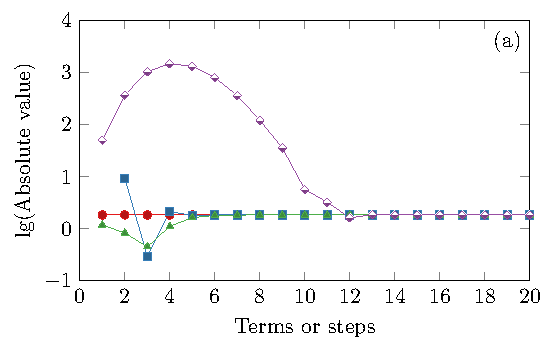
\includegraphics[width = \textwidth]{E:/Research/PistonComp2001/m/sphBessel/fig/compare_jint_200421A_a_200428_v2.pdf}
        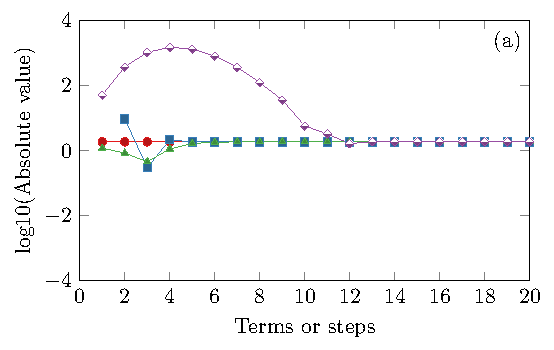
\includegraphics[width = \textwidth]{fig/compare_jint_200421A_a_200428_v3.pdf}
    \end{subfigure}
    \begin{subfigure}{0.49\textwidth}
        \centering
        % \includegraphics[width = \textwidth]{E:/Research/PistonComp2001/m/sphBessel/fig/compare_jint_200421A_b_v2.pdf}
        \includegraphics[width = \textwidth]{fig/compare_jint_200421A_b_v2.pdf}
    \end{subfigure}
    \\
    \begin{subfigure}{0.49\textwidth}
        \centering
        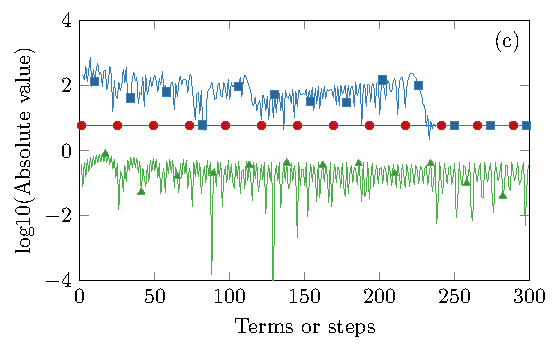
\includegraphics[width = \textwidth]{fig/compare_jint_200421A_c_v2.pdf}
    \end{subfigure}
    \begin{subfigure}{0.49\textwidth}
        \centering
        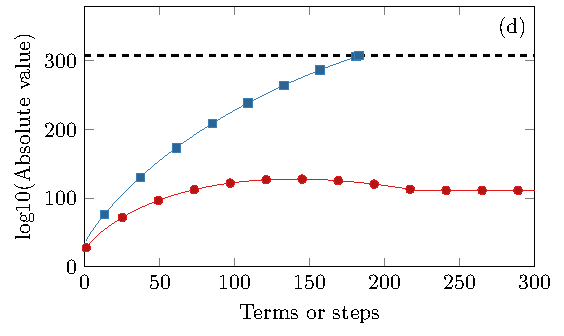
\includegraphics[width = \textwidth]{fig/compare_jint_200421A_d_v2.pdf}
    \end{subfigure}
    \caption{Numerical calculation of the integral \ensuremath{\calJ_{2n}^1(0,ka)} using four methods when (a) $ka = 10$ and $n = 0$; (b) $ka = 300$ and $n = 10$; (c) $ka = 900$ and $n = 10$; and (d) using the GHF series at $n = 10$. {In (a), (b), and (c): red circle, proposed method; blue square, Gauss-Legendre quadrature; green triangle, Bessel expansion; purple diamond, GHF series. In (d): red circle, $ka = 300$; blue square, $ka=900$; dashed line, overflow.
    \revA{The function log10 represents the common logarithm with the base of 10.}}}
    \label{fig:swe_piston_results}
\end{figure}

It can be found in Fig.~\ref{fig:swe_piston_results}(a) that all the results converge rapidly when $ka = 10$, which is in the low frequency range. 
However, the spherical Bessel functions oscillate significantly at large $ka$, so more terms are required in the Gauss-Legendre quadrature and Bessel expansion to obtain accurate results, such as more than 75 and 200 for Gauss-Legendre quadrature in Figs.~\ref{fig:swe_piston_results}(b) and (c), respectively. 
However, only 10 steps are required while using the proposed solution. When the frequency is high, e.g.\ $ka = 300$ or 900, the curve for the GHF series are not included in Figs.~\ref{fig:swe_piston_results}(b) and (c), because the results exceed the vertical axis range. These curves are plotted separately in Fig.~\ref{fig:swe_piston_results}(d) with larger vertical axis ranges. 
The first term of the GHF series of Eq.~(\ref{eq:swe_ghe_series}) is up to $10^{28}$ and $10^{38}$ for $ka = 300$ and 900, respectively, while the accurate results of the integral are only 5.05 and 5.84, respectively.
The result for $ka = 900$ overflows when the truncated terms exceed 183, and the curve for $ka = 300$ converges to an incorrect result much larger than 5.84 due to the loss of significant figures.

The GHF can also be calculated using the built-in function \quotes{hypergeom} in MATLAB where better but not publicly known techniques are used to solve the problems occurred in the direct summation of truncated terms of the GHF series Eq.~(\ref{eq:swe_ghe_series}). 
Table \ref{tab:swe_calc_time} compares the calculation time using the GHF calculated by this built-in function and the proposed method for the orders 0 to $N$, where $N$ is the maximal order required for calculating the sound pressure to give satisfactory precisions. 
The calculation time using the GHF method increases as the $ka$ and $N$ increase and is more than 60 s when $ka = 900$ and $N = 600$, while the time with the proposed method is less than 0.1 s for all cases. 
Furthermore, it is noteworthy that the values calculated by MATLAB are sometimes unreliable and efforts should be spent to validate the accuracy case by case \cite{Pearson2009ComputationHypergeometricFunctions}.

\begin{table}
    \centering
    \begin{tabular}{ccc}
        \toprule
        \multirow{2}{*}{Case}
        & \multicolumn{2}{c}{Calculation time (s)} \\
        \cmidrule(lr){2-3}
        & GHF method & Proposed method\\
        \midrule
        $ka=300$, $N=200$ & 9.47 & 0.0048 \\
        $ka=500$, $N=350$ & 23.12 & 0.016 \\
        $ka = 900$, $N=600$ & 62.75 & 0.043\\
        \bottomrule
    \end{tabular}
    \caption{Comparison of the calculation time when the GHF is calculated by the built-in function \quotes{hypergeom} of MATLAB R2018a (based on \revA{a personal computer with a 2.5 GHz CPU}) and the proposed method.}
    \label{tab:swe_calc_time}
\end{table}


In the following simulations, the common parameters used in modelling audio sound generated by a PAL, are used to verify the accuracy of the proposed solution. 
The radius of the transducer $a = \SI{0.3}{m}$, the frequency $f = \SI{65}{kHz}$, and $ka = 350 + 0.09\rmi$, where the sound speed $c_0 = \SI{343}{m/s}$ and the sound attenuation coefficient in air $\alpha = \SI{0.3}{Np/m}$, which is calculated according to ISO 9613-1 at the temperature of {25\celsius} and the relative humidity of 70\%.

Figure~\ref{fig:swe_piston_soundpressure} shows the normalized sound pressure on the radiation axis of the transducer and the directivity index for the surface velocity profile of the piston ($u_0$) and the simply supported disk $(2u_0[1 - (\rho\subt{s}/a)^2])$.
In the proposed method, the on-axis pressure is calculated by Eq.~(\ref{eq:swe:w9e0fjspd23}) by setting $\theta = 0$, the directivity index is calculated by Eq.~(\ref{eq:swe:w9e0fjspd23}) after using the far field asymptotic formula $\rmh_{2n}(kr) \sim (-1)^n\rmh_0(kr)$ at $kr\to\infty$, 
\begin{equation}
    p(\vb{r},k)
    =
    \rho_0c_0u_0
    \rmh_0(kr)\sum_{n=0}^\infty
    C_{2n}
    P_{2n}(\cos\theta)
    \calJ_{2n}^1 (0,ka)
    % \qty[\int_0^{ka} j_{2n}(t)t \dd t]
    \qc
    kr \to \infty
\end{equation}
and the number of truncated terms is set as 200. The exact values of the on-axis pressure and the directivity index are presented for comparison, which are calculated with Eqs.~(20-21) and Eq.~(29) in \cite{Aarts2009OnaxisFarfieldSound}, respectively. 
The results obtained with the proposed method agree well with those from the exact solutions. 
This validates the accuracy of the proposed method in the exterior region where no closed-form exact solution is available at present. 

\begin{figure}[!htb]
    \centering
    \begin{subfigure}{0.49\textwidth}
        \centering
        % \includegraphics[width = \textwidth]{E:/Research/PistonComp2001/m/rayleigh/fig/compare_prs_200422A_a_v2.pdf}
        \includegraphics[width = \textwidth]{fig/compare_prs_200422A_a_v2.pdf}
    \end{subfigure}
    \begin{subfigure}{0.49\textwidth}
        \centering
        % \includegraphics[width = \textwidth]{E:/Research/PistonComp2001/m/rayleigh/fig/compare_DI_200422A_b_v2.pdf}
        \includegraphics[width = \textwidth]{fig/compare_DI_200422A_b_v2.pdf}
    \end{subfigure}
    \caption{Calculated normalized sound pressure on the radiation axis (a) and the directivity index (b) when $ka = 350 + 0.09\rmi$ for a baffled circular radiator with the uniform (rigid piston) and quadratic (simply supported disk) velocity profiles. {Red circle, rigid piston, proposed method; blue sqaure, rigid piston, exact solution; green triangle, simply supported, proposed method; purple diamond, simply supported, exact solution.}}
    \label{fig:swe_piston_soundpressure}
\end{figure}


\section{SWE for a circular PAL}
\label{sec:swe_pal}
As demonstrated in Chap.~\ref{chap:sound_field},
the ultrasound field is required first to calculate the audio sound field.
In the SWE for a circular PAL, the ultrasound field is calculated using the results given by Eqs.~(\ref{eq:swe:2309fsjdf2}) and (\ref{eq:swe:velocity}) obtained in Sec.~\ref{Section41}.
The SWE for the audio sound field is derived in the following sections.

\subsection{Quasilinear solution of Westervelt equation}
The source density for the virtual audio source at $\vb{r}\subt{v}$ under the spherical coordinate system can be obtained by substituting Eq.~(\ref{eq:swe:2309fsjdf2}) into Eq.~(\ref{eq:source_density_westervelt}), which is 
\begin{equation}
    q(\vb{r}\subt{v})
    =
    \frac{\beta \omega\subt{a}}{\rmi c_0^2}
    \sum_{l,m=0}^\infty
    C_{2l} C_{2m}
    R_{2l}(r\subt{v},k_1)
    R_{2m}^*(r\subt{v},k_2)
    P_{2l}(\cos\theta\subt{v})
    P_{2m}(\cos\theta\subt{v})
    \label{eq:swe:source_density_westervelt}
\end{equation}

The velocity potential for audio sound given by Eq.~(\ref{eq:potential_integral_volume}) can be represented under the spherical coordinates as
\begin{equation}
    \Phi(\vb{r}, k\subt{a})
    = 
    - \int_0^{2\uppi}
    \int_0^\uppi
    \int_0^\infty
    q (\vb{r}\subt{v})
    g(\vb{r},\vb{r}\subt{v}, k\subt{a})
    r\subt{v}^2 \sin\theta\subt{v} 
    \dd r \subt{v} 
    \dd \theta \subt{v}
    \dd \varphi\subt{v}
    \label{eq:swe:suasdop}
\end{equation}
By substituting Eq.~(\ref{eq:swe_green_expansion}) into Eq.~(\ref{eq:swe:suasdop}), 
one obtains
\begin{dmath}
    \Phi(\vb{r},k\subt{a})
    = 
    -\rmi k\subt{a} 
    \sum_{n=0}^\infty
    \sum_{m=-n}^n 
    \qty(n+\frac{1}{2})
    \frac{(n-m)!}{(n+m)!}
    \int_0^\uppi 
    \int_0^\infty
    \rmj_n(k\subt{a}r\subt{v,<})
    \rmh_n(k\subt{a}r\subt{v,>})
    \\ \qquad \times
    P_{n}^m(\cos\theta)
    P_n^m(\cos\theta\subt{s})
    \qty[\frac{1}{2\uppi}
    \int_0^{2\uppi}q(\vb{r}\subt{v})
    \rme^{\rmi m(\varphi-\varphi\subt{v})} \dd \varphi\subt{v}]
    r\subt{v}^2 \sin\theta\subt{v}
    \dd \theta\subt{v}
    \label{eq:swe:3289fjsdjp230fwjefwef}
\end{dmath}
According to Eq.~(\ref{eq:swe:source_density_westervelt}), it is clear the source density $q(\vb{r}\subt{v})$ is \revA{independent of} the azimuth angle $\varphi\subt{v}$. 
We then have 
\begin{equation}
    \frac{1}{2\uppi}
    \int_0^{2\uppi} q(\vb{r}\subt{v}) \rme^{\rmi m(\varphi-\varphi\subt{v})}
    \dd \varphi\subt{v}
    = 
    q(\vb{r}\subt{v}) \delta_{m0}
    \label{eq:swe:289fsdsdp}
\end{equation}
By substituting Eq.~(\ref{eq:swe:289fsdsdp}) into Eq.~(\ref{eq:swe:3289fjsdjp230fwjefwef}), one obtains
\begin{dmath}
    \Phi(\vb{r}, k\subt{a})
    =
    -\rmi k\subt{a}
    \sum_{n = 0}^\infty 
    \qty(n + \frac{1}{2})P_n (\cos\theta)
    \\\times
    \int_{0}^\uppi
    \int_0^\infty 
    q(\vb{r}\subt{v})
    P_n(\cos\theta\subt{v})
    j_n(kr\subt{v,<})
    h_n (kr\subt{v,>})
    r\subt{v}^2 \sin\theta\subt{v}
    \dd r \subt{v} 
    \dd \theta \subt{v}
    \label{eq:swe:398jfsd}
\end{dmath}
By substituting the SWE for source density given by Eq.~(\ref{eq:swe:source_density_westervelt}), Eq.~(\ref{eq:swe:398jfsd}) becomes
\begin{dmath}
        \Phi(\vb{r},k\subt{a})
        =
         -\frac{\beta}{\omega\subt{a}}
        \sum_{l,m,n=0}^\infty
        C_{2l}C_{2m} W_{2l,2m,n} 
        \calR_{2l,2m,n}(r,k\subt{a})
        P_n(\cos\theta)
        \label{eq:s923jfwsep20}
\end{dmath}
where the radial component for audio sound is defined as
\begin{equation}
    \calR_{2l,2m,n}(r,k\subt{a})
    =
    \int_0^\infty R_{2l}(r\subt{v},k_1)
    R_{2m}^*(r\subt{v}, k_2) 
    \rmj_n(k\subt{a}r\subt{v,<} ) 
    \rmh_n (k\subt{a} r\subt{v,>}) 
    k\subt{a}^3 r\subt{v}^2 \dd r\subt{v}
    \label{eq:cwe_audio_radial}
\end{equation}
and the auxiliary notation 
\begin{equation}
    W_{2l,2m,n} = \qty(n+\frac{1}{2})
        \int_0^\uppi P_{2l}(\cos\theta\subt{v})P_{2m}(\cos\theta\subt{v})P_{n}(\cos\theta\subt{v})\sin\theta\subt{v}\dd \theta\subt{v}
        \label{eq:swe:Wigner39280rf}
\end{equation}
By using Eq.~(\ref{eq:legendre:9032rfjsd}), the integral in Eq.~(\ref{eq:swe:Wigner39280rf}) is eliminated and it is expressed using Wigner $3j$ symbol as
\begin{equation}
    W_{2l,2m,n} = 
    \qty(2n+1)
    \mqty(2l & 2m & n \\ 0 & 0 & 0)^2
\end{equation}
According to Eq.~(\ref{eq:p39fsdp9801}), $W_{2l,2m,n} = 0$ when $n$ is odd.
Therefore, Eq.~(\ref{eq:s923jfwsep20}) takes the form of 
\begin{equation}
    \Phi(\vb{r},k\subt{a})
    =
    -\frac{\beta}{\omega\subt{a}}
    \sum_{l,m,n=0}^\infty
    C_{2l} C_{2m} W_{2l,2m,2n}
    \calR_{2l,2m,2n}(r,k\subt{a})P_{2n}(\cos\theta)
    \label{eq:90jsfd12}
\end{equation}

For the special case when the field point is on the $z$ axis, i.e., $\theta = 0$, Eq.~(\ref{eq:90jsfd12}) is reduced to 
\begin{equation}
    \Phi(\vb{r},k\subt{a})
    =
    -\frac{\beta}{\omega\subt{a}}
    \sum_{l,m,n=0}^\infty
    C_{2l} C_{2m} W_{2l,2m,2n}
    \calR_{2l,2m,2n}(r,k\subt{a})
    \label{eq:90jsfd12231}
\end{equation}
by utilizing the fact that $P_{2n}(1) = 1$.

The explicit expressions for the interior and the exterior radial components are 
\begin{dmath}
    \calR \supt{int}_{2l,2m,2n}(r, k\subt{a})
    = 
    \rmh_{2n}(k\subt{a} r) 
    \int_0^r
    R\supt{int}_{2l}(r\subt{v},k_1)
    \qty[R_{2m}\supt{int}(r\subt{v},k_2)]^*
    \rmj_{2n}(k\subt{a}r\subt{v})k\subt{a}^3 r\subt{v}^2 \dd r\subt{v}
    +
    \rmj_{2n}(k\subt{a}r)
    \int_r^a R_{2l}\supt{int}(r\subt{v}, k_1)
    \qty[R_{2m}\supt{int} (r\subt{v},k_2)]^*
    \rmh_{2n}(k\subt{a}r\subt{v})
    k\subt{a}^3 r\subt{v}^2 \dd r\subt{v}
    + \rmj_{2n}(k\subt{a}r)
    \int_a^\infty 
    R_{2l}\supt{ext}(r\subt{v},k_1)
    \qty[R_{2m}\supt{ext}(r\subt{v},k_2)]^*
    \rmh_{2n}(k\subt{a}r\subt{v})
    k\subt{a}^3 r\subt{v}^2 \dd r\subt{v}
    \qc~{r<a}
    \label{eq:spoi4e3fj203}
\end{dmath}

\begin{dmath}
    \calR\supt{ext}_{2l,2m,2n}(r, k\subt{a})
    = 
    \rmh_{2n}(k\subt{a} r)
    \int_0^a R_{2l}\supt{int}(r\subt{v},k_1)
    \qty[R_{2m}\supt{ext} (r\subt{v},k_2)]^*
    \rmj_{2n}(k\subt{a}r\subt{v}) k\subt{a}^3 r\subt{v}^2 \dd r\subt{v}
    + 
    \rmh_{2n}(k\subt{a}r) 
    \int_a^r R_{2l}\supt{ext} (r\subt{v}, k_1)
    \qty[R_{2m}\supt{ext} (r\subt{v},k_2)]^*
    \rmj_{2n}(k\subt{v} r\subt{v})
    k\subt{a} ^3 
    r\subt{v}^2 \dd r\subt{v}
    + \rmj_{2n}(k\subt{a}r)
    \int_r^\infty 
    R_{2l}\supt{ext}(r\subt{v}, k_1)
    \qty[R_{2m}\supt{ext} (r\subt{v},k_2)]^*
    \rmh_{2n}(k\subt{a}r\subt{v})
    k\subt{a}^3 r\subt{v}^2 \dd r\subt{v}\qc~{r>a}
    \label{eq:spoi4e3fj203}
\end{dmath}
respectively. 
It will be shown that only the exterior region
of Eq.~(\ref{eq:spoi4e3fj203}) is required for most scenarios because the interior
region is very small compared to the space of interests.

Equation (\ref{eq:s923jfwsep20}) is the main result of this \revA{section}.
It is an
exact solution to the audio sounds generated by a PAL solved
by the Westervelt function with the quasilinear assumption.
Because no additional assumptions are made in the derivation,
it is equivalent rigorously to the original solution Eq.
(\ref{eq:swe:suasdop}) which has five-fold integrals and is more accurate than
the GBE solution. 
Equation (\ref{eq:s923jfwsep20}) can be calculated more efficiently
for three reasons. 
First, it is a series with threefold
summation consisting of uncoupled spherical angular and
radial components, so it can be calculated quickly for a large
number of field points. Second, the radial component
$\calR_{2l,2m,2n}(r,k\subt{a})$ can be transformed into a rapidly converged integral
using the property of spherical Bessel functions.
Finally, due to the restrictions of the triangular
inequality, many values of Wigner $3j$ symbol are
zero, so many terms do not need to be calculated

\subsection{Quasilinear solution of Kuznetsov equation}
\label{sec:predict_swe_kuz}
When the local effects are considered, the Kuznetsov equation should be used in the mathematical modelling.
The source density for this case is given by Eq.~(\ref{eq:kuznetsov:source:density}).
After expanding the components of the velocity field under the spherical coordinate system, 
 Eq.~(\ref{eq:kuznetsov:source:density}) can be rewritten as a summation of three components
 \begin{equation}
     q(\vb{r}) = q\subt{p}(\vb{r})+ q_r(\vb{r}) + q_\theta(\vb{r})
     \label{eq:2389fjwds239wdof}
 \end{equation}
 where 
 \begin{equation}
     q\subt{p}(\vb{r}) = \frac{(\beta-1)\omega\subt{a}\omega_1\omega_2}{\rmi c_0^4}
     \Phi(\vb{r}, k_1) \Phi^*(\vb{r},k_2)
     \label{eq:qp}
 \end{equation}
 \begin{equation}
     q_r(\vb{r} ) =
     \frac{\omega\subt{a}}{\rmi c_0^2}
     v_r(\vb{r},k_1)v_r^*(\vb{r},k_2)
     \label{eq:qr}
 \end{equation}
 \begin{equation}
     q_\theta(\vb{r})
     =
     \frac{\omega\subt{a}}{\rmi c_0^2}
     v_\theta (\vb{r},k_1) v_\theta^*(\vb{r},k_2)
     \label{eq:qtheta}
 \end{equation}

 Similar to Eq.~(\ref{eq:swe:source_density_westervelt}), we have the SWE for the source density by substituting Eqs.~(\ref{eq:swe:2309fsjdf2} and (\ref{eq:swe:velocity}) into Eqs.~(\ref{eq:qp}), (\ref{eq:qr}), and (\ref{eq:qtheta})
\begin{equation}
 q\subt{p}(\vb{r}\subt{v})
=
\frac{(\beta-1) \omega\subt{a}}{\rmi c_0^2}
\sum_{l,m=0}^\infty
C_{2l} C_{2m}
R_{2l}(r\subt{v},k_1)
R_{2m}^*(r\subt{v},k_2)
P_{2l}(\cos\theta\subt{v})
P_{2m}(\cos\theta\subt{v})
\label{eq:swe:source_density_kuznetsov}
\end{equation}
\begin{equation}
    q_r(\vb{r}\subt{v})
    =
    \frac{\omega\subt{a}}{\rmi c_0^2}
    \sum_{l,m=0}^\infty 
    C_{2l}C_{2m}
    \dv{R_{2l}(r\subt{v},k_1) }{(k_1r\subt{v})}
    \qty[\dv{R_{2m}(r\subt{v},k_2)}{(k_2r\subt{v})}]^* P_{2l}(\cos\theta\subt{v})
    P_{2m}(\cos\theta\subt{v})
\end{equation}
\begin{equation}
    q_\theta(\vb{r}\subt{v})
    =
    \frac{\omega\subt{a}}{\rmi c_0^2}
    \sum_{l,m=0}^\infty 
    C_{2l}C_{2m}
    \frac{R_{2l}(r\subt{v},k_1) }{k_1r\subt{v}}
    \qty[\frac{R_{2m}(r\subt{v},k_2)}{k_2r\subt{v}}]^*
    \dv{P_{2l}(\cos\theta)}{\theta\subt{v}}
    \dv{P_{2m}(\cos\theta\subt{v})}{\theta\subt{v}}
\end{equation}

The velocity potential field of audio sound can then be written as a sum of the contribution from 3 components of virtual source density given on the right-hand side of Eq.~(\ref{eq:2389fjwds239wdof})
\begin{equation}
    \Phi(\vb{r},k\subt{a})
    = \Phi\subt{p}(\vb{r}, k\subt{a})
    + \Phi_r(\vb{r}, k\subt{a})
    + \Phi_\theta(\vb{r},k\subt{a})
    \label{eq:cwe_potential_components}
\end{equation}
Similar to the derivation of Eq.~(\ref{eq:90jsfd12}), the corresponding velocity potential fields are obtained as
\begin{equation}
    \Phi\subt{p}(\vb{r},k\subt{a})
    = 
    -\frac{\beta-1}{\omega\subt{a}}
    \sum_{l,m,n=0}^\infty
    C_{2l}C_{2m}W_{2l,2m,2n}
    \calR_{\rmp, 2l, 2m,2n}(r,k\subt{a})
    P_{2n}(\cos\theta)
    \label{eq:cwe_potential_p}
\end{equation}
\begin{equation}
    \Phi_r(\vb{r}, k\subt{a})
    = -\frac{1}{\omega\subt{a}}
    \sum_{l,m,n=0}^\infty
    C_{2l}C_{2m}W_{2l,2m,2n}
    \calR_{r,2l,2m,2n}(r, k\subt{a})P_{2n}(\cos\theta)
    \label{eq:cwe_potential_r}
\end{equation}
\begin{dmath}
    \Phi_\theta(r,k\subt{a})
    = -\frac{1}{\omega\subt{a}}
    \sum_{l,m,n=0}^\infty
    C_{2l}C_{2m}
    W_{2l,2m,2n}
    \qty[l(2l+1)+m(2m+1)-n(2n+1)]
    \calR_{\theta,2l,2m,2n}(r, k\subt{a})
    P_{2n}(\cos\theta)
    \label{eq:cwe_potential_theta}
\end{dmath}
where we have used the results given by Eq.~(\ref{eq:triple:23908fjs}), \revA{where the integrals of triple Legendre polynomials are derived}.

The triangular inequality
should also be satisfied, so that $\abs{l-m} \leq n \leq l+m$. The
radial components of audio sound $\calR_{2l,2m,2n}(r,k\subt{a})$, $\calR_{r,2l,2m,2n}(r,k\subt{a})$, and $\calR_{\theta,2l,2m,2n}(r,k\subt{a})$
are then given by
\begin{equation}
    \calR_{\rmp, 2l,2m,2n}(r, k\subt{a})
    =
    \int_0^\infty R_{2l}(r\subt{v}, k_1)
    R_{2m}^*(r\subt{v},k_2)
    \rmj_{2n}(k\subt{a} r\subt{v,<})
    \rmh_{2n}(k\subt{a} r\subt{v,>})
    k\subt{a}^3 r^2\subt{v} \dd r\subt{v}
    \label{eq:cwe_R_p}
\end{equation}
\begin{equation}
    \calR_{r,2l,2m,2n}(r, k\subt{a})
    =\int_0^\infty 
    \dv{R_{2l}(r\subt{v},k_1)}{(k_1 r\subt{v})}
    \dv{R_{2m}^*(r\subt{v},k_2)}{(k_2^* r \subt{v})} 
    \rmj_{2n}(k\subt{a},r\subt{v,<})
    \rmh_{2n}(k\subt{a}r\subt{v,>})
    k\subt{a}^3 r\subt{v}^2 \dd r\subt{v}
    \label{eq:cwe_R_r}
\end{equation}
\begin{equation}
    \calR_{\theta,2l,2m,2n}(r,k\subt{a})
    = \int_0^\infty R_{2l}(r\subt{v},k_1)
    R_{2m}^*(r\subt{v},k_2)
    \rmj_{2n}(k\subt{a} r\subt{v,<})
    \rmh_{2n}(k\subt{a} r\subt{v,>})
    \frac{k\subt{a}^3}{k_1k_2^*}
    \dd r\subt{v}
    \label{eq:cwe_R_theta}
\end{equation}
Equations (\ref{eq:cwe_potential_components}) to (\ref{eq:cwe_R_theta}) are the main results of this section.
Equation (\ref{eq:cwe_potential_components}) is solved by the Kuznetsov equation with the quasilinear
assumption and this is exact over the entire field. 
Because no additional assumptions are made in the derivation, it is
equivalent to the original solution to Eq.~(\ref{eq:kuznetsov_p_phi}) that contains
five-fold integrals. 
The proposed expressions in Eqs.~(\ref{eq:cwe_potential_p}) to (\ref{eq:cwe_potential_theta})
 can be calculated more efficiently for three reasons:
(1) it is a series with a threefold summation consisting
of uncoupled spherical angular and radial components; 
(2) the radial components $\calR_{\rmp,2l,2m,2n}(r,k\subt{a})$, $\calR_{r,2l,2m,2n}(r,k\subt{a})$, and $\calR_{\theta,2l,2m,2n}(r,k\subt{a})$ can be transformed into a rapidly converged integral using the property
of spherical Bessel functions ; 
and (3) a number of the terms do not need to be calculated
because many values of the Wigner $3j$ symbol are zero due
to the restrictions of the triangular inequality.

\subsection{Approximation in the inverse-law far field}
\label{sec:swe_pal_inverse_law}
The asymptotic formula for spherical Hankel functions at
$k\subt{a}r\to \infty$ yeilds
\begin{equation}
    \rmh_{2n}(k\subt{a}r) \sim 
    (-1)^n \rmh_0(k\subt{a}r) 
    =
    (-1)^n \frac{\rme^{\rmi k \subt{a} r}}{ \rmi k \subt{a} r}
\end{equation}
so that the radial component given by Eq.~(\ref{eq:cwe_audio_radial}) can be simplified as 
\begin{equation}
    \calR_{2l,2m,2n} (r,k\subt{a})
    = 
    (-1)^n \frac{\rme^{\rmi k \subt{a} r}}{ \rmi k \subt{a} r}
    \int_0^\infty R_{2l}(r\subt{v},k_1)
    R_{2m}^*(r\subt{v}, k_2)
    \rmj_{2n}(k\subt{a}r\subt{v} )
    k\subt{a}^3 r\subt{v}^2 \dd r\subt{v}
    \label{eq:cwe_audio_radial_farfield}
\end{equation}
Equation (\ref{eq:cwe_audio_radial_farfield}) can be calculatd as 
\begin{dmath}
    \calR_{2l,2m,2n}(r, k\subt{a})
    = 
    (-1)^n %h_{0}(k\subt{a} r)
\frac{\rme^{\rmi k \subt{a} r}}{ \rmi k \subt{a} r}
    \int_0^a R_{2l}\supt{int}(r\subt{v},k_1)
    \qty[R_{2m}\supt{int} (r\subt{v},k_2)]^*
    \rmj_{2n}(k\subt{a}r\subt{v}) k\subt{a}^3 r\subt{v}^2 \dd r\subt{v}
    + 
    (-1)^n%h_{0}(k\subt{a} r)
\frac{\rme^{\rmi k \subt{a} r}}{ \rmi k \subt{a} r}
    \int_a^\infty R_{2l}\supt{ext} (r\subt{v}, k_1)
    \qty[R_{2m}\supt{ext} (r\subt{v},k_2)]^*
    \rmj_{2n}(k\subt{v} r\subt{v})
    k\subt{a} ^3 
    r\subt{v}^2 \dd r\subt{v}
    \label{eq:spoi4e3fj20223}
\end{dmath}
which is the limiting form of Eq.~(\ref{eq:spoi4e3fj203}).
By substituting Eq.~(\ref{eq:cwe_audio_radial_farfield}) into Eq.~(\ref{eq:s923jfwsep20}), it is clear that the
audio sound pressure amplitude is inversely proportional to
the propagating distance, $r$, so that the audio sound in the
inverse-law far field is obtained. 
It is noteworthy that the solution obtained here is more accurate than existing ones,
such as the GBE and convolution models introduced in Secs.~\ref{sec:predict_gbe} and \ref{sec:predict_conv}, because the complex nonlinear interactions in the near field of the PAL are more accurately captured.

\subsection{Numerical simulations}
\subsubsection{Validation of the SWE}
To illustrate the accuracy and efficiency of the proposed method, the parameters in \cite{Cervenka2019VersatileComputationalApproach} are used and also listed in Table \ref{tab:swe:pal:parameter}. 
Figure~\ref{fig:swe:pal:valid} shows the audio SPL as a function of the truncated term N at several typical field points when $y = 0$. 
It is clear that all the curves converge with sufficient terms. 
The truncated error is less than 0.1 dB when the truncated term $N$ is larger than 10.

\begin{table}
    \centering
    \begin{tabular}{cc}
        \toprule
        Item	& Value\\
        \midrule
        Average ultrasound frequency	& $f\subt{u} = \SI{39.5}{kHz}$\\
        Audio frequency	& $f\subt{a} = \SI{1}{kHz}$\\
        Sound attenuation coefficients	& $\alpha_1 = \alpha_2 = \SI{2.8e-2}{Np/m}$\\
        Transducer surface radius	&$a = \SI{0.02}{m}$\\
        Helmholtz number	& $k\subt{u}a =14.7$\\
        Rayleigh distance	& $\SI{0.146}{m}$\\
        \bottomrule
    \end{tabular}
    \caption{The parameters used for validating the proposed method in Sec.~\ref{sec:swe_pal}}
    \label{tab:swe:pal:parameter}
\end{table}
\begin{figure}[h]
    \centering
    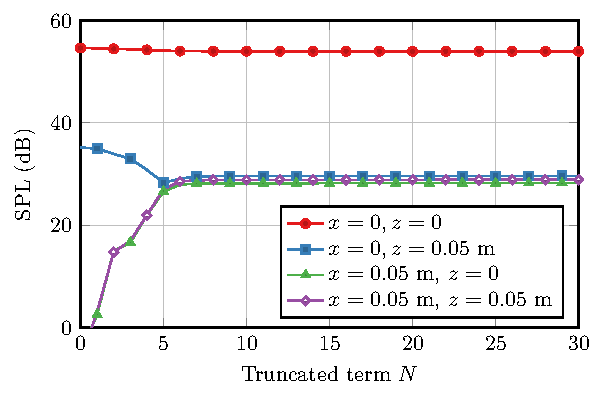
\includegraphics[width = 0.6\textwidth]{Figures/show_TruncatedTerms_200802K_v2.pdf}
    \caption{Convergence of the audio SPL \revA{(dB re 20 $\mu$Pa)} as a function of the truncated term $N$ at several typical field points when $y = 0$, where the parameters in Table \ref{tab:swe:pal:parameter} are used.}
    \label{fig:swe:pal:valid}
\end{figure}

For comparison, the direct integration of Eq.~(\ref{eq:potential_integral_volume}) is performed (denoted by \quotes{direct method}), where the \revA{Simpson's 1/3 rule} is used for numerical integrations. 
\revA{Simpson's 1/3 rule is a classical numerical technique for evaluating integrals, and it was used here because it is quick and sufficiently accurate for this particular integral. This approach was verified by ensuring the numerical integration converged.}
The integrated coordinates are evenly discretized, and the field coordinate is set as the middle point between adjacent integrated coordinates to avoid singularities of Green's functions. 
The infinitely large integral domain is reduced to a cylindrical column centered along the axis of the PAL with a radius of 1.5 m and a length of 3 m to cover the major energy of ultrasonic beams. 

Figure~\ref{fig:verification:f2w90fs} shows the audio SPL as a function of the propagating distance in different directions at 1 kHz, where the results obtained by the proposed method are same as that from the direct method. 
But the proposed method is faster than the direct method to calculate the audio sound in different directions because the polar angle coordinate, $\theta$, of the field point is uncoupled in the expression. 
For example, the radial components in Eqs.~(\ref{eq:cwe_R_p}) to (\ref{eq:cwe_R_theta}) need to be calculated only once when obtaining the 3 curves in Fig.~\ref{fig:verification:f2w90fs}.

\begin{figure}[h]
    \centering
    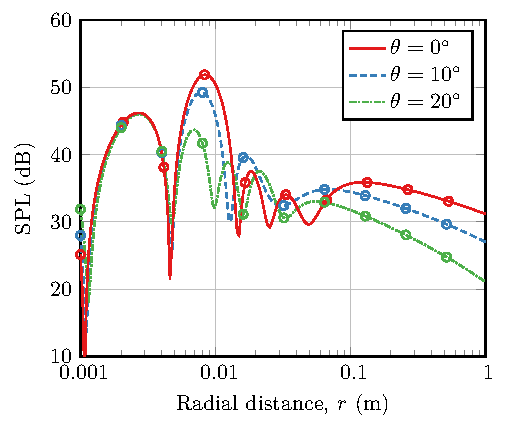
\includegraphics[width = 0.5\textwidth]{Figures/pending/compare_Cervenka2019JASA_diffAngle_200802F.pdf}
    \caption{The audio SPL \revA{(dB re 20 $\mu$Pa)} as a function of the propagating distance in different directions at 1 kHz, where the circles are that obtained by using the direct method. 
    \revA{Solid line, $\theta = 0^\circ$; dashed line, $\theta = 10^\circ$; dash dotted line, $\theta = 20^\circ$.}}
    \label{fig:verification:f2w90fs}
\end{figure}

Table~\ref{tab:swe:time:comparison} lists the computation time of the \revA{proposed SWE and direct integration methods} at 3 typical field points. 
The precision criterion is used to identify the difference between the SPL calculated with the two methods to be less than 0.05 dB. 
The calculation was conducted on a personal computer witha 2.5 GHz CPU and 16 GB random access memory. 
Table \ref{tab:swe:time:comparison} demonstrates that the computation time of the \revA{proposed SWE method} remains similar for all the cases, but is at least 100 times faster than the \revA{direct integration method}. 
The reason for the computation saving is that the direct integration method has to calculate the sound pressure of the ultrasound at many virtual source points and then integrate over a large space, but this is not required in the SWE method.
\begin{table}
    \centering
    \begin{tabular}{ccc}
        \toprule
        \multirow{2}{*}{Field point coordinates} &  \multicolumn{2}{c}{Caclulation time (s)} \\
        \cmidrule(lr){2-3}                       & \revA{SWE method}
                                                 & \revA{Direct integration method} \\
        \midrule
        On-axis $(x,y,z) = (0,0,\SI{0.05}{m}) $ & 0.59 & 75.2\\
        Off-axis $(x,y,z) = (\SI{0.05}{m}, 0, \SI{0.05}{m})$ & 0.56 & 82.5 \\
        On the PAL $ (x,y,z) = 0$ & 0.64 & 354.6\\
        \bottomrule
    \end{tabular}
    \caption{\revA{Comparison of the calculation time of the SWE method and the direct integration method.}}
    \label{tab:swe:time:comparison}
\end{table}

\subsubsection{The transition distance from the near field to the Westervelt far field}
\label{sec:cwe_transition_near_westervelt}
Figure~\ref{fig:swep:389fs} shows the audio SPL at 1 kHz and the ultrasound field at 40 kHz on the radiation axis as a function of the propagating distance, where the transducer radius is 0.05 m. 
The ultrasound pressure is calculated with the closed-form formula given by Eq.~(\ref{eq:piston:axis:closed_form}) 
\begin{equation}
    \scrL(z,k\subt{u})
    =
    \frac{\rho_0}{2}v_z^2(z,k\subt{u})
    -
    \frac{p^2(z,k\subt{u})}{2\rho_0c_0^2}
    \label{eq:ultra:lagrangian_density}
\end{equation}
where $v_z(z,k\subt{u})$ is the particle velocity component in $z$ direction and can be obtained by the relation $v_z(z,k\subt{u}) = (\rmi k\subt{u} \rho_0c_0)^{-1}\pdv*{p(z,k\subt{u})}{z}$
\begin{equation}
    v_z(z,k\subt{u})
    =
    u_0
    \rme^{\rmi k\subt{u}z}
    -u_0
    \frac{z}{a}
    \qty(1+\frac{z^2}{a^2})^{-1/2}
    \exp\qty(\rmi k\subt{u} a \sqrt{1+\frac{z^2}{a^2}})
\end{equation}
The obtained ultrasound pressure and Lagrangian density on the radiation axis are then normalized by $2\rho_0c_0u_0$ and $2\rho_0u_0$, respectively, and are shown in Fig.~\ref{fig:swep:389fs}(b).
\begin{figure}[h]
    \centering
    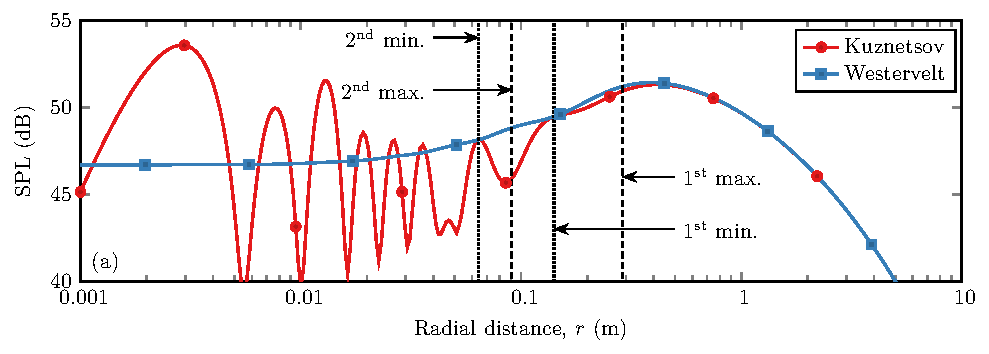
\includegraphics[width = 0.95\textwidth]{Figures/pending/show_nearfield_radius0p05_ultra40e3_audio1000_200725D.pdf}
    \caption{Audio SPL \revA{(dB re 20 $\mu$Pa)} at 1 kHz  as a function of the propagating distance on the radiation axis, where the transducer radius is 0.05 m}
    \label{fig:swep:389fs}
\end{figure}
\begin{figure}[h]
    \centering
    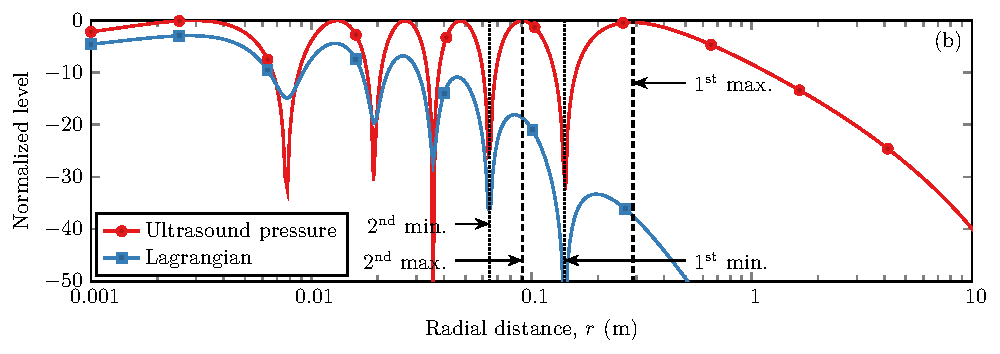
\includegraphics[width = 0.95\textwidth]{Figures/pending/show_nearfield_radius0p05_ultra40e3_axis_200725H.pdf}
    \caption{The level of normalized ultrasound pressure and Lagrangian density at the average ultrasound frequency 40 kHz.}
    \label{fig:wefpsd03}
\end{figure}

The ultrasound pressure amplitude has several local minima and maxima in the near field. From Eq.~(\ref{eq:piston:axis:closed_form}), the radial distance at the local minima can be obtained by, see Eq.~(5.7.4) in~\cite{Pierce2019AcousticsIntroductionIts}
\begin{equation}
    r\subt{min}(n)
    = 
    \qty[\qty(\frac{a}{\lambda\subt{u}})^2 - n^2]
    \frac{\lambda\subt{u}}{2n}
    \qc
    n =
    1,2, \ldots,
    \left\lfloor \frac{a}{\lambda\subt{u}} \right\rfloor
    \label{eq:swe_rmin}
\end{equation}
where $\lambda\subt{u}$ is the wavelength at the average ultrasound frequency $f\subt{u}$ and $\lfloor \cdot \rfloor$ rounds down the quantity inside. Similarly, the radial distance at the local maxima can be obtained by

\begin{equation}
    r\subt{max}(n)
    =
    \qty[\qty(\frac{a}{\lambda\subt{u}})^2 - 
    \qty(n-\frac{1}{2})^2]
    \frac{\lambda\subt{u}}{2n-1}
    \qc
    n=1,2,\ldots,
    \left\lfloor
        \frac{a}{\lambda\subt{u}}+\frac{1}{2}
    \right\rfloor
    \label{eq:swe:rmax}
\end{equation}
The first two ($n$ = 1 and 2) local minima and maxima are plotted in Figs.~\ref{fig:swep:389fs} and \ref{fig:wefpsd03}. 
It appears that the locations of local maxima and minima of ultrasonic Lagrangian density are close to that of the ultrasound pressure.

The ultrasonic Lagrangian density is non-cumulative as the propagation of the ultrasound beams \cite{Aanonsen1984DistortionHarmonicGeneration}.
In the near field, where the field point is close to a PAL, the ultrasonic Lagrangian density fluctuates significantly, and the audio sound calculated with the Kuznetsov equation in Fig.~\ref{fig:swep:389fs} is complicated which means that the results obtained with the Westervelt equation are inaccurate. 
Figure~\ref{fig:wefpsd03} shows that the ultrasonic Lagrangian density is small when the radial distance is larger than the first local maximum (0.29 m in this case), and the results calculated with the Westervelt equation in Fig.~\ref{fig:swep:389fs} are also accurate.

The transition from the near field to the Westervelt far field is affected by the local minima and maxima of the ultrasound pressure amplitude. 
As shown in in Fig.~\ref{fig:wefpsd03}, at the first two local minima, the normalized Lagrangian density is more than 30 dB lower than that near the PAL, so it can be neglected in the calculation of audio sounds and the results obtained by the Kuznetsov and Westervelt equations are almost the same.
At the distance of the first two local maxima, the Lagrangian density amplitude is near its local maxima, 
so its effects are prominent and the difference between the results obtained by the Kuznetsov and Westervelt equations is large. 
The difference decreases as the ordinal number of the local maximum decreases. 
For example, the difference is 3.0 dB at the second local maximum (0.09 m) and it decreases to 0.3 dB at the first local maximum (0.29 m).

Figures~\ref{fig:kuznetsov:diff_ultra_freq} shows the difference of the audio SPL calculated with the Kuznetsov and Westervelt equations as a function of the propagating distance on the radiation axis, with different transducer radii at different ultrasound frequencies for an audio frequency of 1 kHz. 
The radial distance to the first maximum of the ultrasound pressure amplitude is listed in Table~\ref{tab:maxima:near_field_to_westervelt_field} and calculated by setting $n = 1$ in Eq.~(\ref{eq:swe:rmax}), so that
\begin{equation}
    r\subt{max}(1)
    = 
    \frac{a^2}{\lambda\subt{u}}
    -
    \frac{\lambda\subt{u}}{4}
\end{equation} 
At large radial distances, the audio SPL difference approaches 0 dB indicating the accuracy of using the Westervelt equation. At small radial distances, the number of local minima and maxima increases as the transducer radius and ultrasound frequency increases, as predicted from Eqs.~(\ref{eq:swe_rmin}) and (\ref{eq:swe:rmax}).
\begin{figure}[!htb]
    \centering
    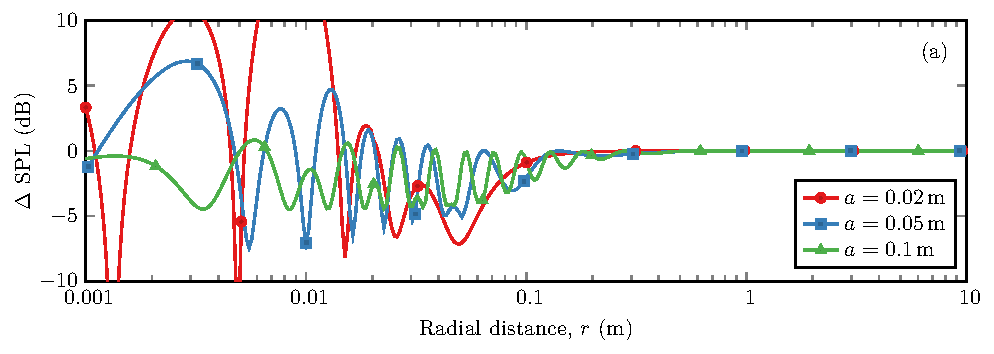
\includegraphics[width = 0.95\textwidth]{Figures/pending/compare_WD_radiusVary_ultra40e3_audio1000_200725A4.pdf}
    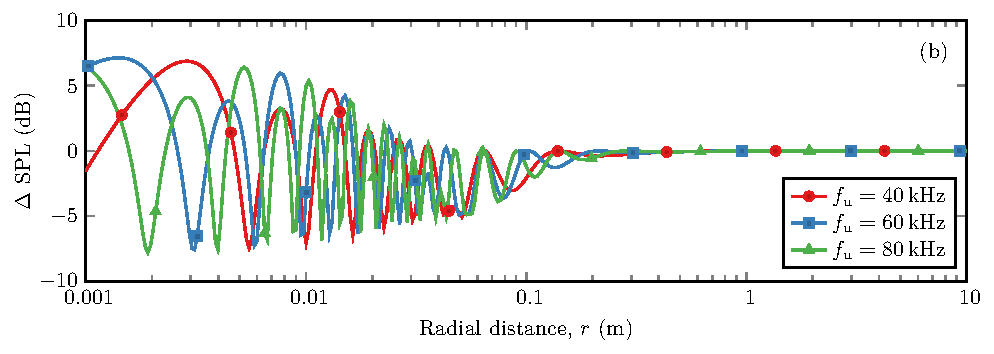
\includegraphics[width = 0.95\textwidth]{Figures/pending/compare_nearfield_radius0p05_ultraVary_audio1000_200725C.pdf}
    \caption{\revA{The audio SPL difference calculated with the Kuznetsov and Westervelt equations as a function of the propagating distance on the radiation axis (a) with different transducer radii when the average ultrasound frequency is 40 kHz, and (b) at different average ultrasound frequencies when the transducer radius is 0.05 m, where the audio frequency is 1 kHz.}}
    \label{fig:kuznetsov:diff_ultra_freq}
\end{figure}

\begin{table}
    \centering
    \begin{tabular}{p{0.13\textwidth}p{0.22\textwidth}p{0.165\textwidth}p{0.38\textwidth}}
        \toprule
        Transducer radius \revA{$a$} (m) & Ultrasound frequency $f\subt{u}$ (kHz) & First maximum $r\subt{max}(1)$ (m) & Transition distance from the near field to the   Westervelt far field (m) \\
        \midrule
        0.02          & 40                            & 0.04                      & 0.04 ($n_0 = 1$)                                                             \\
0.05                  & 40                            & 0.29                      & 0.29 ($n_0 = 1$)                                                             \\
0.1                   & 40                            & 1.16                      & 0.38 ($n_0 = 2$)                                                             \\
0.15                  & 40                            & 2.62                      & 0.51 ($n_0 = 3$)                                                             \\
0.2                   & 40                            & 4.67                      & 0.65 ($n_0 = 4$)                                                             \\
0.25                  & 40                            & 7.29                      & 0.79 ($n_0 = 5$)                                                             \\
0.05                  & 60                            & 0.44                      & 0.44 ($n_0 = 1$)                                                             \\
0.05                  & 80                            & 0.58                      & 0.19 ($n_0 = 2$)                                                             \\
0.05                  & 100                           & 0.73                      & 0.24 ($n_0 = 2$)                                                             \\
        \bottomrule
    \end{tabular}
    \caption{The first maxima of the ultrasound pressure amplitude and the transition distances from the near field to the Westervelt far field for several sets of parameters.}
    \label{tab:maxima:near_field_to_westervelt_field}
\end{table}

The distance at the $n$\mbox{-th} local maximum of the ultrasound pressure amplitude increases as the transducer radius and ultrasound frequency increase, 
where $n$ is any positive integer number restricted by the condition in Eq.~(\ref{eq:swe:rmax}). 
The audio SPL difference at the location of the corresponding local maximum decreases if the transducer radius and ultrasound frequency increase. 
This is because the ultrasound beam is more collimated when the transducer radius and the ultrasound frequency are larger. 
The ultrasound beams can also be approximated by plane waves when they are highly collimated. 
In this case, the ultrasonic Lagrangian density $\scrL$ approaches zero after substituting the plane wave condition $p(z,k\subt{u}) = \rho_0c_0|v_z(z,k\subt{u})|$  into Eq.~(\ref{eq:ultra:lagrangian_density}), 
which means the local effects are negligible and the Westervelt equation is accurate. 
Therefore, the magnitude of the audio SPL difference can be determined by how much the ultrasound beams behave like plane waves, 
which is measured by defining an error function as
\begin{equation}
    \oldeps(z) = 
    \qty[1-\frac{\rho_0c_0 |v_z(z,k\subt{u})|}{\abs{p_z(z,k\subt{u})}}]
    \times 
    100\%
    \label{eq:swe:error_function}
\end{equation}
If the error function is small, the ultrasound beams are more collimated and the effects of the ultrasonic Lagrangian density would also be small.

Because the audio SPL difference calculated with the two equations is large at points near the local maxima of the ultrasound pressure amplitude, 
the transition distance from the near field to the Westervelt far field can be defined as the distance at the $n_0$\mbox{-th} local maximum of the ultrasound pressure amplitude, 
such that the error function at this point is less than a threshold $\oldeps_0 > 0$. 
To obtain $n_0$, the following condition should be satisfied as
\begin{equation}
    \oldeps\qty[r\subt{max}(n_0)]
    \leq \oldeps_0
    \label{eq:swe:eps0}
\end{equation}
The substitution of Eqs.~(\ref{eq:swe:rmax}) and (\ref{eq:swe:error_function}) into Eq.~(\ref{eq:swe:eps0}), $n_0$ is obtained by
\begin{equation}
    n_0
    =
    \max\qty(1,
    \left\lfloor
    \frac{a}{\lambda\subt{u}} \frac{1}{\sqrt{\oldeps_0^{-1}} - 1} + \frac{1}{2}\right \rfloor)
\end{equation}
where $\max(1, \cdot)$ is used to ensure $n_0$ is at least 1. 
The choice of a smaller threshold for $\oldeps_0$ leads to higher precision when using the Westervelt equation to predict audio sounds in the Westervelt far field, 
region $r\geq r\subt{max}(n_0)$. 
The transition distance at several sets of parameters are listed in Table~\ref{tab:maxima:near_field_to_westervelt_field1} when $\oldeps_0 = 2.5\%$, 
and the numerical simulations show the error using the Westervelt equation is less than 0.6 dB under this condition.

Figure~\ref{fig:swe:audio_spl:diff_audio_freq} shows the audio SPL difference at different audio frequencies when the transducer radius is 0.05 m, and the average ultrasound frequency is 40 kHz. 
At high audio frequencies, the audio SPL difference is small at small radial distances. 
This is because the audio SPL calculated with the Westervelt equation increases by about 12 dB when the audio frequency is doubled, 
but the amplitude of the ultrasonic Lagrangian density changes little at different audio frequencies, 
so its effect on the audio SPL is relatively small at high audio frequencies. 
The locations of local minima and maxima in the ultrasound pressure amplitude do not change at different audio frequencies, so the transition distance from the near field to the Westervelt far field does not vary with the audio frequency.
\begin{figure}[!htb]
    \centering
    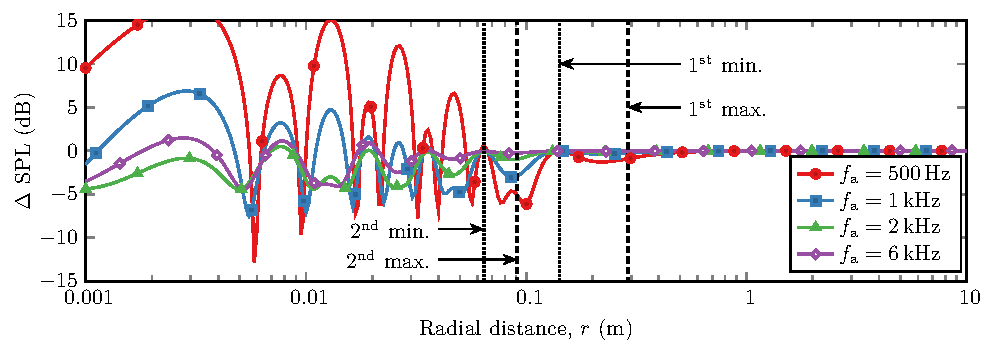
\includegraphics[width = 0.95\textwidth]{Figures/pending/compare_nearfield_radius0p05_ultra40e3_audioVary_200725B}
    \caption{The audio SPL difference calculated with the Kuznetsov and Westervelt equations as a function of the propagating distance on the radiation axis at different audio frequencies (transducer radius is 0.05 m and the average ultrasound frequency is 40 kHz).}
    \label{fig:swe:audio_spl:diff_audio_freq}
\end{figure}

In this section, the formula of the transition distance from the near field to the Westervelt far field is derived based on the transducer with a uniform velocity profile. 
For other velocity profiles such as parabolic and quartic ones \cite{Cervenka2019VersatileComputationalApproach}, an appropriate formula can be obtained using a method similar to the one described above. For a specific velocity profile, the key step is to find the location of the local maxima of ultrasound pressure amplitude on the transducer axis, where the Lagrangian density amplitude is large and the local effects are significant.

\subsubsection{The transition distance from the Westervelt far field to the inverse-law far field}
\label{sec:predict_swe_transi_far}
Figure~\ref{fig:swe:farfield} shows the difference between the audio SPL calculated with the Westervelt equation and the inverse-law property, 
as a function of the propagating distance on the radiation axis with different transducer radii at different ultrasound and audio frequencies. 
This difference increases as the radial distance increases, 
and then decreases and approaches 0 dB at large radial distances, 
where the prediction based on the inverse-law property is accurate. 
Taking 1 dB as the error bound, this defines the region where the audio SPL difference is less than 1 dB to be the inverse-law far field. 
Table~\ref{tab:maxima:near_field_to_westervelt_field1} lists the transition distances from the Westervelt far field to the inverse-law far field for the parameters used in Fig.~\ref{fig:swe:farfield}.

\begin{figure}[h]
    \centering
    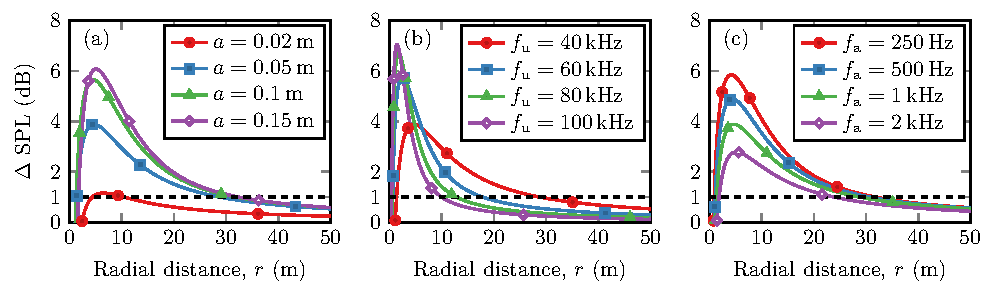
\includegraphics[width = 0.95\textwidth]{Figures/pending/farfield_200803A.pdf}
    \caption{The audio SPL difference calculated with the Westervelt equation and the inverse-law property as a function of the propagating distance on the radiation axis (a) with different transducer radii when the average ultrasound frequency is 40 kHz and the audio frequency is 1 kHz, (b) at different average ultrasound frequencies when the transducer radius is 0.05 m and the audio frequency is 1 kHz, and (c) at different audio frequencies when the transducer radius is 0.05 m and the average ultrasound frequency is 40 kHz, where ΔSPL = 1 dB for the dashed lines.}
    \label{fig:swe:farfield}
\end{figure}
\begin{table}
    \centering
    \begin{tabular}{p{0.14\textwidth}p{0.17\textwidth}p{0.18\textwidth}p{0.32\textwidth}}
        \toprule
        Transducer radius $a$ (m) & Ultrasound frequency $f\subt{u}$ (kHz) & Audio frequency $f\subt{a}$ (Hz) & Inverse-law transition distance (m) when $\Delta \mathrm{SPL} < \SI{1}{dB}$ \\
        \midrule
        
0.02                    & 40                            & 1000                    & 10.6                                                           \\
0.05                    & 40                            & 1000                    & 29.1                                                           \\
0.1                     & 40                            & 1000                    & 31.8                                                           \\
0.15                    & 40                            & 1000                    & 33.0                                                           \\
0.05                    & 60                            & 1000                    & 17.8                                                           \\
0.05                    & 80                            & 1000                    & 12.8                                                           \\
0.05                    & 100                           & 1000                    & 10.2                                                           \\
0.05                    & 40                            & 250                     & 32.3                                                           \\
0.05                    & 40                            & 500                     & 30.6                                                           \\
0.05                    & 40                            & 2000                    & 23.9                                                          \\
        \bottomrule
    \end{tabular}
    \caption{The transition distance from the Westervelt far field to the
inverse-law far field for the parameters.}
    \label{tab:maxima:near_field_to_westervelt_field1}
\end{table}

Figure~\ref{fig:swe:farfield}(a) shows that the transition distance increases as the transducer radius increases. 
For example, it increases from 10.6 m to 29.1 m as the transducer radius increases from 0.02 m to 0.05 m. 
This is because the effective virtual source containing the major ultrasonic energy becomes larger as the transducer radius increases. 
Figure~\ref{fig:swe:farfield}(b) shows that the transition distance decreases as the ultrasound frequency increases. 
For example, it decreases from 29.1 m to 17.8 m when the ultrasound frequency increases from 40 kHz to 60 kHz. 
This is because the effective virtual source becomes smaller as the sound attenuation coefficient of ultrasound beams in air becomes larger. 
Although the transition distance decreases as the audio frequency increases Fig.~\ref{fig:swe:farfield}(c), the effects are relatively small. 
For example, it decreases by only 1.5 m ($4.9\%$) when the audio frequency increases from 500 Hz to 1 kHz.

The effects of the transducer radius, and the ultrasound and audio frequencies on the inverse-law transition distance, are more complicated than the one from the near field to the Westervelt far field. 
It seems that the ultrasound frequency is the most important parameter because the ultrasound attenuation coefficient in air changes significantly as the frequency and meteorological conditions change. 
Therefore, an empirical formula, for example $4/\alpha\subt{u}$, 
can be used to estimate the inverse-law far field transition distance, where αu is the ultrasound attenuation coefficient in air at the average ultrasound frequency $f\subt{u}$. 
The physical meaning of this formula is that the ultrasound pressure amplitude at this location has been attenuated to $2\% (\rme^{-4} \approx 0.02)$. 
However, the formula does not hold for the very small sound absorption coefficient.

\section{Cylindrical wave expansion (CWE) for a phased array source}
\label{sec:cwe_source}

\subsection{Theory}
The model considered in this section is shown in Fig.~\ref{fig:pal2d:model}.
A rectangular coordinate system $(x,y,z)$ and a cylindrical coordinate system $(\rho,\varphi,z)$ is used for reference.

To express Eq.~(\ref{eq:potential_2d}) as a cylindrical expansion, the addition theorem for the Hankel function is introduced, so that \cite{Poletti2019CylindricalExpansionsSound, Williams1999FourierAcousticsSound}
\begin{equation}
    H_0(k |\bm{\uprho}_1-\bm{\uprho}\subt{2}|)
    = \sum_{n=-\infty}^\infty J_n(k \rho_<)H_n(k \rho_>) \rme^{\rmi n (\varphi_1-\varphi_2)}
    \label{eq:hankel_expansion}
\end{equation}
where $J_n(\cdot)$ is the Bessel function of order $n$, $H_n(\cdot)$ is the Hankel function of order 0, $\rho_{<} = \min(\rho_1,\rho_2)$ and $\rho_>=\max(\rho_1,\rho_2)$.

For the source point on the positive $x$ axis, $x\subt{s} = \rho\subt{s}$ and $\varphi\subt{s} =0 $; 
for the source point on the negative $x$ axis, $x\subt{s} = -\rho\subt{s}$ and $\varphi\subt{s} = \uppi$ . 
Substituting Eq.~(\ref{eq:hankel_expansion}) into Eq.~(\ref{eq:potential_2d}) yields
\begin{equation}
    \Phi(\bm{\uprho},k) = \frac{1}{2\rmi k}
    \sum_{n=-\infty}^\infty R_n(\rho, k) \rme^{\rmi n \varphi}
    \label{eq:cwe_potential}
\end{equation}
where the radial component is expressed as
\begin{equation}
    R_n(\rho,k)
    = \int_0^a J_n(k\rho\subt{s,<})
    H_n(k\rho\subt{s,>} )
    u(\rho\subt{s}, k)k\dd \rho\subt{s}
    + \rme^{-\rmi n \uppi}
    \int_0^a J_n(k\rho\subt{s,<} )
    H_n(k\rho\subt{s,>})
    u(-\rho\subt{s}, k)
    k\dd \rho\subt{s}
    \label{eq:cwe_radial_component0}
\end{equation}
where $\rho\subt{s,<}=\min(\rho,\rho\subt{s})$ and $\rho\subt{s,>}=\max(\rho,\rho\subt{s})$.
By introducing the substitution 
\begin{equation}
    u_n(\rho\subt{s}, k) = u(\rho\subt{s}, k)
    +(-1)^n u (-\rho\subt{s},k)
\end{equation}
Eq.~(\ref{eq:cwe_radial_component0}) is rewritten in a more compact form 
\begin{equation}
    R_n(\rho,k) = \int_0^a J_n(k\rho\subt{s,<})
    H_n(k\rho\subt{s,>} ) 
    u_n(\rho\subt{s}, k) 
    k\dd \rho\subt{s}
    \label{eq:cwe_ultra_radial}
\end{equation}

It is easy to show that 
\begin{equation}
    u_{-n}(\rho\subt{s},k) = u(\rho\subt{s},k) + (-1)^{-n} u(-\rho\subt{s},k)
    = u(\rho\subt{s},k) + (-1)^n u(-\rho\subt{s},k) = u_n(\rho\subt{s},k)
    \label{eq:8923asjdf}
\end{equation}
\begin{equation}
    J_{-n}(\cdot) H_{-n}(\cdot) = J_n(\cdot)H_n(\cdot)
    \label{eq:1289fjws9d8f}
\end{equation}
Therefore, the symmetry property of the radial component given by Eq.~(\ref{eq:cwe_ultra_radial}) yields
\begin{equation}
    R_{-n}(\rho,k) = R_n(\rho,k)
    \label{eq:rad:2930fjwsd}
\end{equation}
The substitution of
\begin{equation}
    \rme^{\rmi n \varphi} + \rme^{-\rmi n \varphi } = 2\cos n\varphi
\end{equation}
into Eq.~(\ref{eq:cwe_potential}) yields another form of the velocity potential without the negative order terms
\begin{equation}
    \Phi(\bm{\uprho},k)
    =\frac{1}{2\rmi k}
    \sum_{n=0}^\infty \eps_n R_n(\rho,k)\rme^{\rmi n \varphi}
    \label{eq:2389fga9r8ef2w}
\end{equation}
where $\eps_n$ is the Neumann factor, $\eps_n = 1$ when $n=0$ and $\eps_n = 2$ when $n = 1,2,3,\ldots$.


Similar to Eqs.~(\ref{eq:swe:29jwe03278fjsd}) and (\ref{eq:cwe_radial_ext}), Eq.~(\ref{eq:cwe_ultra_radial}) can be written in the interior and exterior parts as
\begin{equation}
    R_{n}(\rho,k)
    =
    \begin{dcases}
        R_{n}\supt{int}(\rho,k), &\rho < a\\
        R_n\supt{ext}(\rho,k) , & \rho > a
    \end{dcases}
    \label{eq:ae23f90sd}
\end{equation}
with 
\begin{equation}
    R_n\supt{int}(\rho,k)
    =
    H_n(k\rho)\int_0^{k\rho }u(t/k,k)J_n(t)\dd t 
    + 
    J_n(k\rho) \int_{k\rho}^{ka} u(t/k,k) H_n(t)\dd t
    \label{eq:2390rjasd023jdfjap}
\end{equation}
\begin{equation}
    R_n\supt{ext}(\rho,k)
    =
    H_n(k\rho) \int_0^{ka} u(t/k,k) J_n(t)\dd t 
    \label{eq:cwe_radial_ext23}
\end{equation}

To obtain the directivity of the ultrasound used in the convolution method in Eq.~(\ref{eq:conv}), the radial component in Eq.~(\ref{eq:cwe_ultra_radial}) can be simplified using the limiting forms of the Hankel functions for large arguments, see Eq.~(5.1.17) in \cite{Zhang1996ComputationSpecialFunctions}, so that
\begin{equation}
    \lim_{\rho\to\infty} R_n(\rho, k)
    =
    \sqrt{\frac{2}{\uppi k\rho}}
    \frac{\rme^{\rmi k\rho}}{\rmi^{n+1/2}}
    \int_0^a 
    J_n(k\rho\subt{s} )
    u_n (\rho\subt{s}, k)k\dd \rho\subt{s}
    \label{eq:cwe_ultra_radial_far}
\end{equation}


The components of the velocity field under the cylindrical coordiante system can be obtained directly from Eq.~(\ref{eq:cwe_potential}) to give
\begin{equation}
    \begin{dcases}
        v_\rho (\bm{\uprho}, k) 
        = \pdv{\Phi(\bm{\uprho},k)}{\rho}
        =
        \frac{1}{2\rmi }\sum_{n=-\infty}^\infty 
        \dv{R_n(\rho,k)}{(k\rho)} 
        \rme^{\rmi n \varphi}\\
        v_\varphi(\bm{\uprho},k)
        = 
        \frac{1}{\rho}
        \pdv{\Phi(\bm{\uprho}, k)}{\varphi}
        = 
        \frac{1}{2}
        \sum_{n=-\infty}^\infty
        \frac{R_n(\rho,k)}{k\rho}
        n\rme^{\rmi n \varphi}\\
        v_z(\bm{\uprho}, k ) = 
        \pdv{\Phi(\bm{\uprho},k)}{z}
        =
        0
    \end{dcases}
    \label{eq:21031023012}
\end{equation}

Similarly, Eq.~(\ref{eq:21031023012}) can be represented as
\begin{equation}
    \begin{dcases}
    v_\rho(\bm{\uprho},k) = \frac{1}{2\rmi} \sum_{n=0}^\infty \eps_n \dv{R_n(\rho,k)}{(k\rho)}\cos(n\varphi)\\
    v_\varphi(\bm{\uprho},k) = \frac{\rmi }{2} \sum_{n=0}^\infty 
    n\eps_n \frac{R_n(\rho,k)}{k\rho} \sin(n\varphi)\\
    v_z(\bm{\uprho},k) = 0
    \end{dcases}
    \label{eq:289fe982jjjj}
\end{equation}

The derivative of the radial component is required to calculate in Eqs.~(\ref{eq:21031023012}) and (\ref{eq:289fe982jjjj}).
The radial components in interior and exterior regions can be obtained using Eqs.~(\ref{eq:2390rjasd023jdfjap}) and (\ref{eq:cwe_radial_ext23}), respectively, to give
\begin{equation}
    \dv{R_n\supt{int}(\rho,k)}{(k\rho)}
    =
    H'_n(k\rho)\int_0^{k\rho }u(t/k,k)J_n(t)\dd t 
    + 
    J'_n(k\rho) \int_{k\rho}^{ka} u(t/k,k) H_n(t)\dd t
    \label{eq:2390rjasd023jdfja32p}
\end{equation}
\begin{equation}
    \dv{R_n\supt{ext}(\rho,k)}{(k\rho)}
    =
    H'_n(k\rho) \int_0^{ka} u(t/k,k) J_n(t)\dd t 
    \label{eq:cwe_radial_ext2133}
\end{equation}

\subsection{The radial component}


As shown in the radial component given by Eqs.~(\ref{eq:2390rjasd023jdfjap}) and (\ref{eq:cwe_radial_ext23}), the numerical calculation of the integral over Bessel and Hankel functions is required.
The uniform velocity profile, $u(\rho,k) = u_0$, is the most common one.
For covenience, the auxiliary integrals are defined as
\begin{equation}
    \calJ_n(x) = \int J_n(x)\dd x
    \label{eq:12123}
\end{equation}
\begin{equation}
    \calH_n(x) = \int H_n(x) \dd x
    \label{eq:320242}
\end{equation}

The following recurrence relation holds for both Bessel and Hankel functions, see Eq.~(5.1.24) in \cite{Zhang1996ComputationSpecialFunctions}
\begin{equation}
    J_{n+1}(x) = J_{n-1}(x)-2J_n'(x)
    \label{eq:bessel_recurrence}
\end{equation}
Therefore, it is easy to obtain that 
\begin{equation}
    \calJ_{2n+1}(x) = \calJ_1(x) - \sum_{m=1}^n J_{2m}(x)
    \label{eq:123sdf1}
\end{equation}
According to the recurrence relation between orders 0 and 1 for Bessel functions
\begin{equation}
    J'_0(x) = -J_1(x)
    \label{eq:bew02}
\end{equation}
Equation (\ref{eq:123sdf1}) is reduced to 
\begin{equation}
    \calJ_{2n+1}(x) = -\sum_{m=0}^n \eps_m J_{2m}(x)
    \label{eq:12304}
\end{equation}
Similar to Eq.~(\ref{eq:123sdf1}), it can be obtained for the even orders as
\begin{equation}
    \calJ_{2n}(x) = \calJ_0(x) - 2 \sum_{m=1}^n J_{2m-1}(x)
    \label{eq:123234013}
\end{equation}
According to Eq.~(\ref{eq:123040210}), Eq.~(\ref{eq:123234013}) is expressed as
\begin{equation}
    \calJ_{2n}(x) = \frac{\uppi x}{2} \qty[J_1(x)\vb{H}_0(x) - J_0(x)\vb{H}_1(x)] + xJ_0(x)
    - 2\sum_{m=1}^n J_{2m-1}(x)
    \label{eq:13012412310}
\end{equation}
where $\vb{H}_n(\cdot)$ is the Struve function of order $n$.


\section{CWE for a phased array PAL}
\label{sec:cwe_pal}
\subsection{Quasilinear solution of Westervelt equation}
This section aims to obtain the quasilinear solution of Westervelt equation by using the CWE method.
The substitution of Eqs.~(\ref{eq:green_2d_328}) and (\ref{eq:hankel_expansion}) into the potential for audio sound given by Eq.~(\ref{eq:chap3:902jfd}) yields
\begin{equation}
    \Phi(\bm{\uprho},k\subt{a})
    = \frac{1}{4\rmi }
    \sum_{l=-\infty}^\infty
    \int_0^{2\uppi}
    \int_0^\infty
    q(\bm{\uprho}\subt{v})
    J_l(k\rho\subt{v,<})
    H_l(k\rho\subt{v,>})
    \rme^{\rmi l (\varphi-\varphi\subt{v})}
    \rho\subt{v}
    \dd\rho\subt{v}
    \dd\varphi\subt{v}
    \label{eq:12031mfsd}
\end{equation}
where $\rho\subt{v,<} = \min(\rho,\rho\subt{v})$ and $\rho\subt{v,>} = \max(\rho,\rho\subt{v})$.

Substituting Eq.~(\ref{eq:cwe_potential}) into the source density of the audio sound given by Eq.~(\ref{eq:source_density_westervelt}), one obtains the cylindrical expansion at the virtual source point $\bm{\uprho}\subt{v}$ as
\begin{equation}
    q(\bm{\uprho}\subt{v}) = \frac{\beta\omega\subt{a}}{4\rmi c_0^2}
    \sum_{m,n=-\infty}^\infty
    R_m(\rho\subt{v},k_1)R_n^*(\rho\subt{v},k_2)
    \rme^{\rmi (m-n)\varphi\subt{v}}
    \label{eq:cwe_src_density_expansion}
\end{equation}
The substitution of Eq.~(\ref{eq:cwe_src_density_expansion}) into Eq.~(\ref{eq:12031mfsd}) yields
\begin{equation}
    \begin{split}
        \Phi(\bm{\uprho},k\subt{a})
        = 
        -\frac{\beta\uppi }{8 \omega\subt{a}}
        & \sum_{l,m,n=-\infty}^\infty
        \rme^{\rmi l \varphi}
        \times
        \qty[\frac{1}{2\uppi} \int_0^{2\uppi} \rme^{\rmi (m-n-l)\varphi\subt{v}}\dd \varphi\subt{v}]\\
        &\times 
        \int_0^\infty 
        R_m(\rho\subt{v},k_1)
        R_n^*(\rho\subt{v}, k_2)
        J_l(k\subt{a}, \rho\subt{v,<})
        H_l(k\subt{a}, \rho\subt{v,>})
        k\subt{a}^2 \rho\subt{v}
        \dd \rho\subt{v}
    \end{split}
    \label{eq:cwe_potential0}
\end{equation}
\revA{Only those terms that are present when $l=m-n$ are retained in Eq.~({\ref{eq:cwe_potential0}}) because}
\begin{equation}
    \frac{1}{2\uppi} \int_0^{2\uppi}
    \rme^{\rmi(m-n-l)\varphi\subt{v}}\dd \varphi\subt{v}
    =
    \begin{dcases}
        1, & l= m-n\\
        0, & l\neq m-n
    \end{dcases}
\end{equation}
The audio sound pressure may then be reduced to a cylindrical expansion, which yields
\begin{equation}
    \Phi(\bm{\uprho},k\subt{a})
    =
    -\frac{\beta\uppi }{8\omega\subt{a} }
    \sum_{m,n=-\infty}^\infty
    \calR_{mn}(\rho,k\subt{a})
    \rme^{\rmi(m-n)\varphi}
    \label{eq:cwe_audio}
\end{equation}
where the radial component for audio sound is expressed as 
\begin{equation}
    \calR_{mn}(\rho,k\subt{a}) = \int_0^\infty R_m(\rho\subt{v},k_1)R_n^* (\rho\subt{v},k_2)
    J_{m-n}(k\subt{a},\rho\subt{v,<})H_{m-n}(k\subt{a}\rho\subt{v,>})
    k\subt{a}^2 \rho\subt{v}
    \dd \rho\subt{v}
    \label{eq:cwe_audio_radial_component}
\end{equation}
According to Eq.~(\ref{eq:cwe_audio_radial_component}), it is observed when $m, n\geq 0$, the following symmetric relations hold 
\begin{equation}
    \calR_{-m,-n} (\rho, k\subt{a})
    =
    \calR_{m,n}(\rho,k\subt{a})
    \label{eq:18832904}
\end{equation}
\begin{equation}
    \calR_{-m,n} (\rho, k\subt{a})
    =
    \calR_{m,-n}(\rho,k\subt{a})
    \label{eq:1228832904}
\end{equation}
Equation (\ref{eq:cwe_audio}) can then be simplified as
\begin{equation}
    \Phi(\bm{\uprho},k\subt{a})
    =
    -\frac{\beta\uppi }{8\omega\subt{a} }
    \sum_{m,n=0}^\infty
    \eps_{m+n}\qty[\calR_{mn}(\rho,k\subt{a})
    \cos(m-n)\varphi + \calR_{m,-n}(\rho,k\subt{a}) \cos(m+n)\varphi]
    \label{eq:23890199222}
\end{equation}



\subsection{Quasilinear soultion of Kuznetsov equation}
This section aims to obtain the quasilinear solution of Kuznetsov equation by using the CWE method.
Similar to the discussion in Sec.~\ref{sec:predict_swe_kuz}, after expanding the components of the velocity field under the cylindrical coordinate system, the sourcen density given by Eq.~(\ref{eq:kuznetsov_p_phi}) can be rewritten as a summation of three components 
\begin{equation}
    q(\bm{\uprho})
    =
    q\subt{p}(\bm{\uprho})
    +
    q_\rho(\bm{\uprho})
    + 
    q_\varphi(\bm{\uprho})
    \label{eq:123012039}
\end{equation}
where
\begin{equation}
    q\subt{p}(\bm{\uprho})
    = 
    \frac{(\beta-1)\omega\subt{a}\omega_1\omega_2}{ \rmi c_0^4}
    \Phi(\bm{\uprho},k_1)\Phi^*(\bm{\uprho},k_2)
    \label{eq:21301203124218}
\end{equation}
\begin{equation}
    q_\rho(\bm{\uprho})
    =
    \frac{\omega\subt{a} }{\rmi c_0^2}
    v_\rho(\bm{\uprho},k_1)
    v_\rho^*(\bm{\uprho},k_2)
    \label{eq:1203102344}
\end{equation}
\begin{equation}
    q_\varphi(\bm{\uprho})
    =
    \frac{\omega\subt{a}}{ \rmi c_0^2}
    v_\varphi(\bm{\uprho},k_1)
    v_\varphi^*(\bm{\uprho},k_2)
    \label{eq:2101111}
\end{equation}

Similar to Eq.~(\ref{eq:cwe_src_density_expansion}), we have the CWE for the sourcen density by substituting Eqs.~(\ref{eq:cwe_potential}) and (\ref{eq:21031023012}) into Eqs.~(\ref{eq:21301203124218}), (\ref{eq:1203102344}), and (\ref{eq:2101111}) 
\begin{equation}
    q\subt{p}(\bm{\uprho}\subt{v})
    =
    \frac{(\beta-1)\omega\subt{a}}{4\rmi c_0^2}
    \sum_{m,n=-\infty}^\infty
    R_m(\rho\subt{v},k_1)
    R_n^*(\rho\subt{v},k_2)
    \rme^{\rmi(m-n)\varphi}
    \label{eq:10238488}
\end{equation}
\begin{equation}
    q_\rho(\bm{\uprho}\subt{v})
    =
    \frac{\omega\subt{a}}{4\rmi c_0^2}
    \dv{R_m(\rho\subt{v},k_1)}{(k_1\rho\subt{v})}
    \qty[\dv{R_n(\rho\subt{v},k_2)}{(k_2\rho\subt{v})}]^*
    \rme^{\rmi(m-n)\varphi\subt{v}}
    \label{eq:12032999}
\end{equation}
\begin{equation}
    q_\varphi(\bm{\uprho}\subt{v})
    =
    \frac{\omega\subt{a}}{4\rmi c_0^2}
    \sum_{m,n=-\infty}^\infty
    \frac{R_m(\rho\subt{v},k_1)}{k_1\rho\subt{v}}
    \qty[\frac{R_n(\rho\subt{v},k_2)}{k_2\rho\subt{v}}]^*
    mn
    \rme^{\rmi (m-n)\varphi\subt{v}}
    \label{eq:11111111113}
\end{equation}
The velocity potential field of audio sound can then be written as a sum of the contribution
from 3 components of virtual source density given on the right-hand side of Eq.~(\ref{eq:123012039})
\begin{equation}
    \Phi(\bm{\uprho},k\subt{a})
    =
    \Phi\subt{p}(\bm{\uprho}, k\subt{a})
    +
    \Phi_\rho(\bm{\uprho}, k\subt{a})
    +
    \Phi_\varphi(\bm{\uprho}, k\subt{a})
    \label{eq:10vcjdf023}
\end{equation}
Similar to the derivation of Eq.~(\ref{eq:cwe_audio}), 
the corresponding velocity potential fields are obtained as
\begin{equation}
    \Phi\subt{p}(\bm{\uprho},k\subt{a})
    =
    -\frac{(\beta-1)\uppi }{8\omega\subt{a} }
    \sum_{m,n=-\infty}^\infty
    \calR_{\rmp,mn}(\rho,k\subt{a})
    \rme^{\rmi(m-n)\varphi}
    \label{eq:31249fd}
\end{equation}
\begin{equation}
    \Phi_\rho(\bm\rho,k\subt{a})
    =
    -\frac{\uppi}{8\omega\subt{a}}
    \sum_{m,n=-\infty}^\infty
    \calR_{\rho,mn}(\rho,k\subt{a})
    \rme^{\rmi (m-n)\varphi}
    \label{eq:12310fdp}
\end{equation}
\begin{equation}
    \Phi_\varphi(\bm\rho,k\subt{a})
    =
    -\frac{\uppi}{8\omega\subt{a}}
    \sum_{m,n=-\infty}^\infty
    mn
    \calR_{\rho,mn}(\rho,k\subt{a})
    \rme^{\rmi (m-n)\varphi}
    \label{eq:30fdfp2}
\end{equation}

The radial components of audio sound are given by 
\begin{equation}
    \calR_{\rmp,mn}(\rho,k\subt{a})
    = \int_0^\infty R_m(\rho\subt{v},k_1)R_n^* (\rho\subt{v},k_2)
    J_{m-n}(k\subt{a},\rho\subt{v,<})H_{m-n}(k\subt{a}\rho\subt{v,>})
    k\subt{a}^2 \rho\subt{v}
    \dd \rho\subt{v}
    \label{eq:2103fasdp92}
\end{equation}
\begin{equation}
    \calR_{\rho,mn}(\rho,k\subt{a})
    = \int_0^\infty \dv{R_m(\rho\subt{v},k_1)}{(k_1\rho\subt{v})}
    \dv{R_n^* (\rho\subt{v},k_2)}{(k_2^* \rho\subt{v})}
    J_{m-n}(k\subt{a},\rho\subt{v,<})
    H_{m-n}(k\subt{a}\rho\subt{v,>})
    k\subt{a}^2 \rho\subt{v}
    \dd \rho\subt{v}
    \label{eq:1231dfasdj}
\end{equation}
\begin{equation}
    \calR_{\varphi,mn}(\rho,k\subt{a})
    = \int_0^\infty 
    R_m(\rho\subt{v},k_1)
    R_n^* (\rho\subt{v},k_2)
    J_{m-n}(k\subt{a},\rho\subt{v,<})H_{m-n}(k\subt{a}\rho\subt{v,>})
    \frac{ k\subt{a}^2 }{k_1k_2^* \rho\subt{v}}
    \dd \rho\subt{v}
    \label{eq:2103fasdp922}
\end{equation}




\subsection{Approximation in the inverse-law far field}
In the far field, Eq.~(\ref{eq:cwe_audio_radial_component}) has the limiting form
\begin{equation}
    \lim_{\rho\to \infty}
    \calR_{mn}(\rho,k\subt{a})
    =
    \sqrt{\frac{2}{\uppi k\subt{a} \rho}}
    \frac{\rme^{\rmi k\subt{a}\rho}}{\rmi^{m-n+1/2}}
    \int_0^\infty 
    R_m(\rho\subt{v},k_1)
    R_n^*(\rho\subt{v},k_2)
    J_{m-n}(k\subt{a},\rho\subt{v})
    k\subt{a}^2 \rho\subt{v}\dd\rho\subt{v}
    \label{eq:cwe_audio_radial_far}
\end{equation}
As the main result of this section, the cylindrical expansion of the audio sound given by Eq.~(\ref{eq:cwe_audio}) consists of a series of two summations with the uncoupled radial and angular components, 
so it can be calculated quickly for many field points. 
It can be seen as a two-dimensional version of the spherical expansion as developed in Sec.~\ref{sec:swe_pal}, which is a series of triple summations. 
It has been demonstrated the calculation of the spherical expansion is more than 100 times faster than the direct integration of the fivefold in Eq.~(\ref{eq:potential_integral_volume}). 
The cylindrical expansion is simpler than the spherical expansion, so the computational efficiency is further improved. 
In addition, arbitrary excitation velocity profiles, $u(x,k_i)$, can be assumed for the ultrasound source in the radial component for ultrasound given by Eq.~(\ref{eq:cwe_ultra_radial}), so it can be used to model a phased array PAL.

\subsection{Velocity profiles for a steerable PAL}
In this section, a steerable PAL is used as an example of the proposed cylindrical expansion, which aims to steer the audio beam in a desired direction. 
The phased array technique assumes that an excitation of an array of PALs consists of an amplitude and a phase at each PAL unit \cite{Shi2014OverviewDirectivityControl}.

For the ideal configuration, when the size of the PAL unit is infinitely small, a continuous velocity profile can be assumed as
\begin{equation}
    u(x,k_i) = u_0\rme^{\rmi k_ia\cos\varphi_0}
    \label{eq:cwe_vel0}
\end{equation}
whre $u_0$ is a constant with the unit of m/s, and $\varphi_0$ is the steering angle so that $0\leq \varphi_0\leq \uppi$.

For the non-ideal configuration, when the PAL unit has a finite size of $a_0$ (also known as the sub-array size), 
the phase distribution on the radiation surface of each unit must be uniform. 
Therefore, the discrete profile is given by a relation to the continuous one as
\begin{equation}
    u\subt{dis}(x,k_i)
    =
    u\qty(\qty(\left \lfloor \frac{x}{a_0} + \frac{1}{2}\right \rfloor ) a_0, k_1)
    \label{eq:cwe_vel_dis}
\end{equation}

In real applications, the separation between the centers of adjacent PAL units may be larger than their size to give a blank region on the rigid baffle \cite{Shi2015ConvolutionModelComputing, SchmerrJr2014FundamentalsUltrasonicPhased}. 
This can be modelled by multiplying the profiles in Eqs.~(\ref{eq:cwe_vel0}) and (\ref{eq:cwe_vel_dis}) with a weighting function such that the weight is zero in the blank region, which reads
\begin{equation}
    A(x)
    =
    \begin{dcases}
        1, & -\frac{a_1}{2} \leq x - \qty(\left\lfloor \frac{x}{a_0} + \frac{1}{2} \right \rfloor +\frac{1}{2}) a_0
        \leq \frac{a_1}{2}\\
        0, & \text{otherwise}
    \end{dcases}
\end{equation}
where $a_1$ is the separation between the centers of the adjacent PAL units.

To better understand the continuous and discrete velocity profiles for a steerable PAL, Fig.~\ref{fig:cwe_velocity_profile} shows a comparison between them for amplitudes and phases. 
The parameters used are the same as in Fig.~\cite{Shi2014OverviewDirectivityControl, Shi2015ConvolutionModelComputing}: the PAL is steered at $70^\circ$ with a carrier frequency of 40 kHz; 
the phased array PAL size is $2a =\SI{ 0.1}{m}$; the size of each PAL unit is $a_0 = \SI{0.01}{m}$; and the separation of the centers of adjacent units is $a_1 =\SI{ 0.0125}{m}$.

\begin{figure}[!htb]
    \centering
    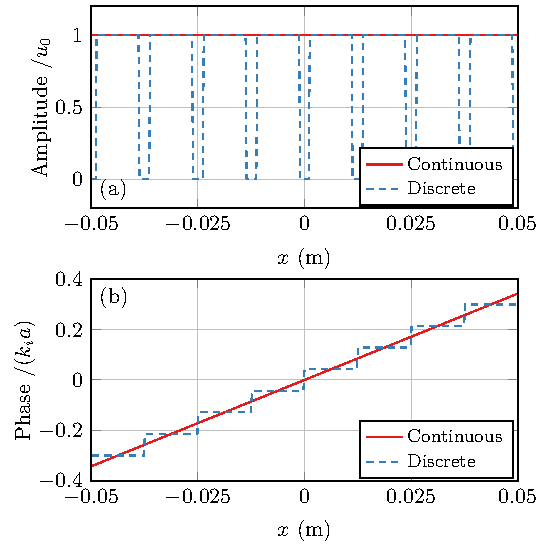
\includegraphics[width = 0.5\textwidth]{fig/VelocityProfile_211023D}
    \caption{Comparison of the continuous and discrete velocity profile for the ultrasound: (a) normalized amplitude distribution, and (b) normalized phase distribution.}
    \label{fig:cwe_velocity_profile}
\end{figure}

\subsection{Results and discussions}
\label{sec:cwe_results}
The cylindrical expansion of the audio sound in Eq.~(\ref{eq:cwe_potential}) is a series which must be truncated to obtain numerical results. 
The truncation limit is set to 70 for both m and n in the following simulations, which delivers an error of less than 0.1 dB for the parameters used in this section. 
The onefold integral in Eqs.~(\ref{eq:cwe_ultra_radial}) and (\ref{eq:cwe_audio_radial_component}) are calculated using the classical Gauss-Legendre quadrature method, although the computation efficiency can be further improved using the series expression and the complex plane method \cite{Zhong2020SphericalExpansionAudio, Poletti2019CylindricalExpansionsSound}. 
The sound attenuation coefficients for both ultrasound and audio sound are estimated according to ISO 9613 \cite{1993ISO961311993}. 
The directivities of the ultrasound used in Eq.~(\ref{eq:conv}) of the convolution model are obtained using the cylindrical expansion in Eq.~(\ref{eq:cwe_potential}) with the limiting form of the radial component at large arguments in Eq.~(\ref{eq:cwe_ultra_radial_far}).

To compare against experimental data in the literature, the parameters are set to be the same as those in \cite{Shi2015ConvolutionModelComputing}. 
The center frequency of the ultrasound is 40 kHz, and all the SPLs in the following simulations are normalized, with a maximum of 0 dB to aid comparison.

\subsubsection{Conventional PAL with a uniform excitation}
In this section, a continuous uniform velocity profile is assumed, as this best represents a conventional PAL. 
Figure~\ref{fig:cwe_result_2d} shows the audio sound fields generated by a conventional PAL with a size of $2a = \SI{0.08}{m}$ at 500 Hz, 1 kHz, 2 kHz, and 4 kHz. 
The results are obtained using the proposed cylindrical expansion. 
It is observed that the main lobe of the generated audio beam is on the radiation axis so that $\varphi = 90^\circ$, and the beam becomes more focused as the frequency increases. 

\begin{figure}[!htb]
    \centering
    \begin{subfigure}{0.45\textwidth}
        \centering
        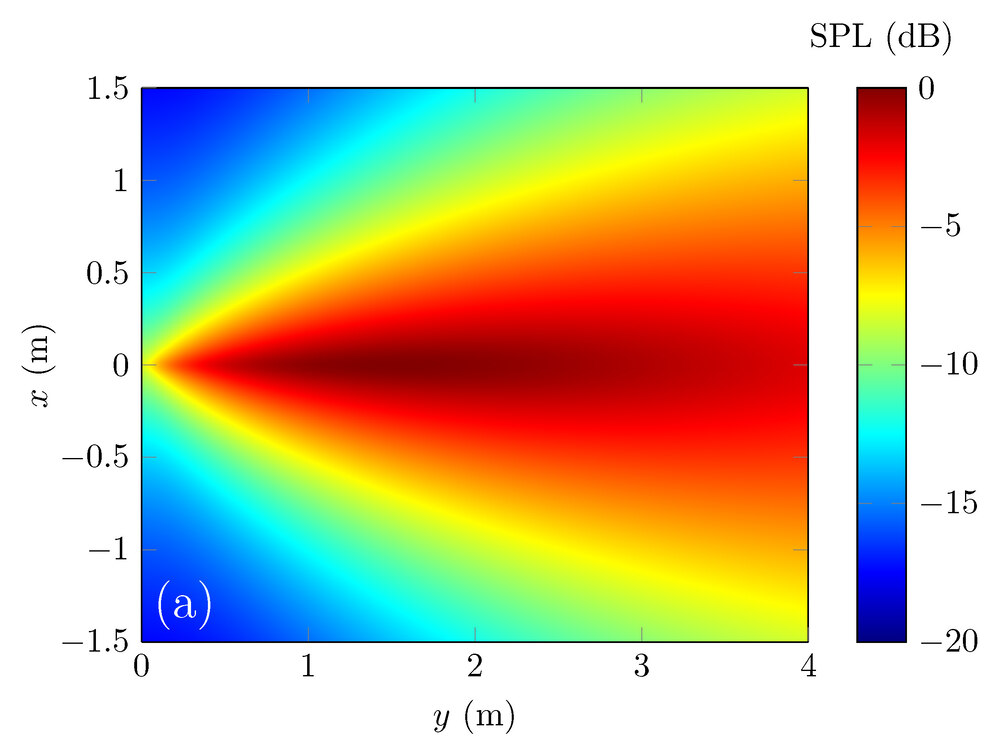
\includegraphics[width = \textwidth]{fig/Shi2015JasaFig4_Pal2D_PWE_Fullfield_Show_500Hz_v3_resize.jpg}
    \end{subfigure}
    \begin{subfigure}{0.45\textwidth}
        \centering
        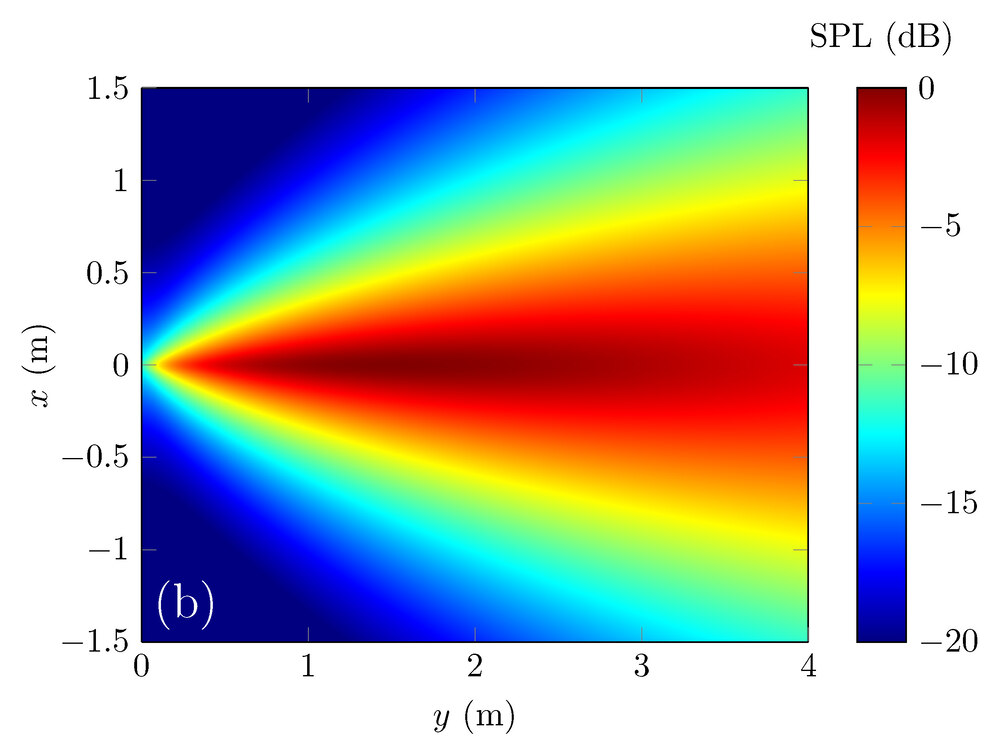
\includegraphics[width = \textwidth]{fig/Shi2015JasaFig4_Pal2D_PWE_Fullfield_Show_1000Hz_v3_resize.jpg}
    \end{subfigure}
    \\
    \begin{subfigure}{0.45\textwidth}
        \centering
        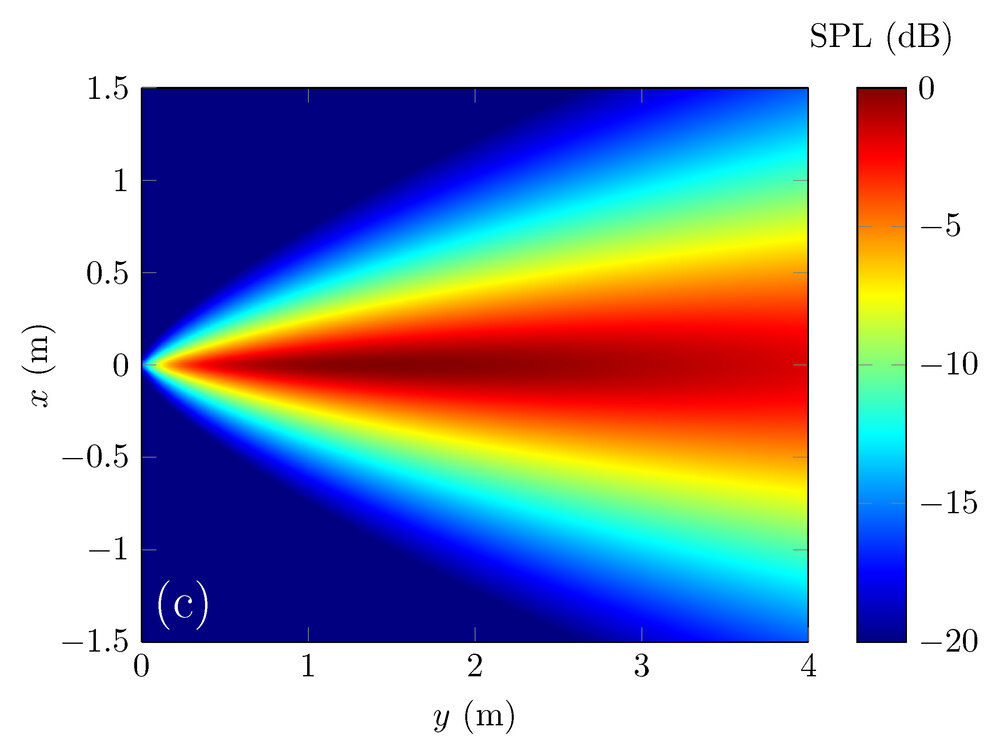
\includegraphics[width = \textwidth]{fig/Shi2015JasaFig4_Pal2D_PWE_Fullfield_Show_2000Hz_v3_resize.jpg}
    \end{subfigure}
    \begin{subfigure}{0.45\textwidth}
        \centering
        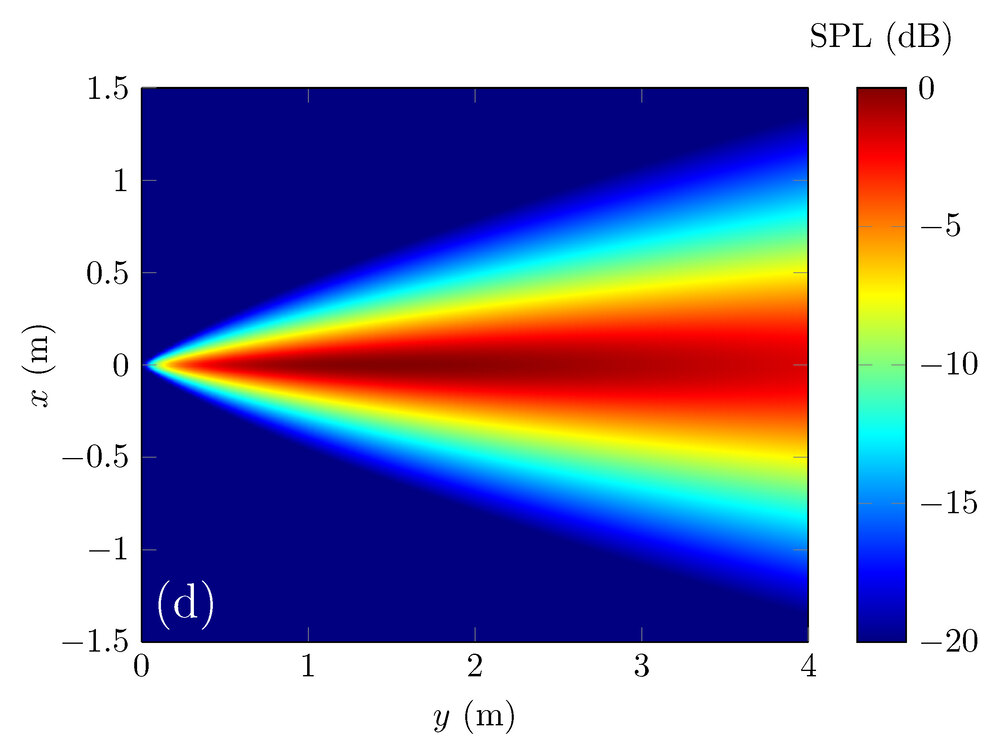
\includegraphics[width = \textwidth]{fig/Shi2015JasaFig4_Pal2D_PWE_Fullfield_Show_4000Hz_v3_resize.jpg}
    \end{subfigure}
    \caption{Audio \revA{SPL (dB re 20 $\mu$Pa)} generated by a conventional PAL with a uniform profile and a size of 0.08 m at (a) 500 Hz, (b) 1 kHz, (c) 2 kHz, and (d) 4 kHz.}
    \label{fig:cwe_result_2d}
\end{figure}

The directivity of the audio sound beam in the far field at different angles and frequencies is shown in Fig.~\ref{fig:cwe_result_compare} using the far field solution of the cylindrical expansion [Eqs.~(\ref{eq:cwe_audio}) and (\ref{eq:cwe_audio_radial_far})]. 
Because the sound pressure was measured at \revA{4 m} away from the PAL in \cite{Shi2015ConvolutionModelComputing}, the results at a radial distance of \revA{4 m} are calculated using the cylindrical expansion [Eqs.~(\ref{eq:cwe_audio}) and (\ref{eq:cwe_audio_radial_component})], and these are also presented in Fig.~\ref{fig:cwe_result_compare}. 
It is interesting to note that the difference between these two curves is large at most angles. 
For example, the difference at $70^\circ$ is 3.3 dB, 2.7 dB, 1.7 dB, and 2.1 dB, at 500 Hz, 1 kHz, 2 kHz, and 4 kHz, respectively. 
It indicates that \revA{4 m} cannot be regarded as far enough away from this PAL source. 
This is because the assumptions and approximations made in the far field imply that the observation point should be far away from the virtual source of the audio sound rather than the radiation surface of the PAL, and this is usually more than \revA{10 m} away, as demonstrated in \cite{Zhong2021FieldWesterveltFar}. 
Therefore, only those results at a radial distance of \revA{4 m} obtained using the cylindrical expansion are presented in the following figures. 

\begin{figure}[!htb]
    \centering
    \begin{subfigure}{0.45\textwidth}
        \centering
        % \includegraphics[width = \textwidth]{E:/Research/Pal2D2108/matlab/fig/Shi2015JasaFig4_500Hz_Compare_v3.pdf}
        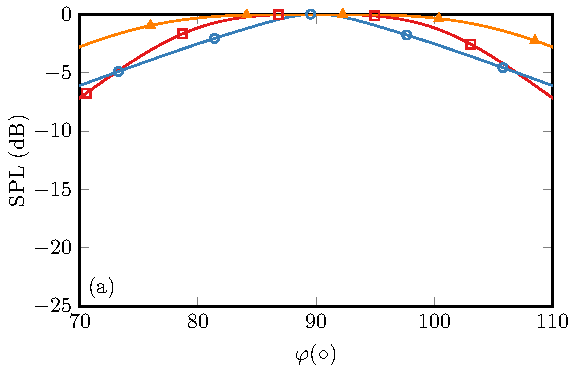
\includegraphics[width = \textwidth]{fig/Shi2015JasaFig4_500Hz_Compare_v3_211014C.pdf}
    \end{subfigure}
    \begin{subfigure}{0.45\textwidth}
        \centering
        % \includegraphics[width = \textwidth]{E:/Research/Pal2D2108/matlab/fig/Shi2015JasaFig4_1000Hz_Compare_v3.pdf}
        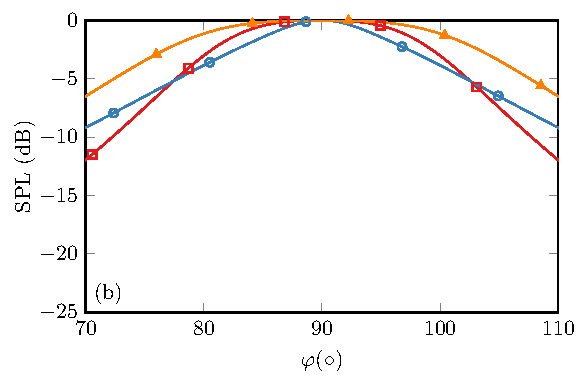
\includegraphics[width = \textwidth]{fig/Shi2015JasaFig4_1000Hz_Compare_v3_21014D.pdf}
    \end{subfigure}
    \\
    \begin{subfigure}{0.45\textwidth}
        \centering
        % \includegraphics[width = \textwidth]{E:/Research/Pal2D2108/matlab/fig/Shi2015JasaFig4_2000Hz_Compare_v3.pdf}
        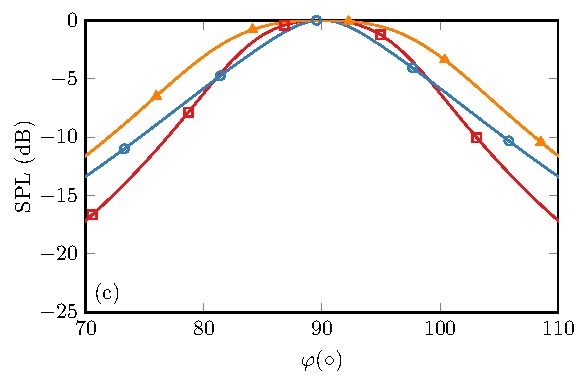
\includegraphics[width = \textwidth]{fig/Shi2015JasaFig4_2000Hz_Compare_v3_211014E.pdf}
    \end{subfigure}
    \begin{subfigure}{0.45\textwidth}
        \centering
        % \includegraphics[width = \textwidth]{E:/Research/Pal2D2108/matlab/fig/Shi2015JasaFig4_4000Hz_Compare_v4.pdf}
        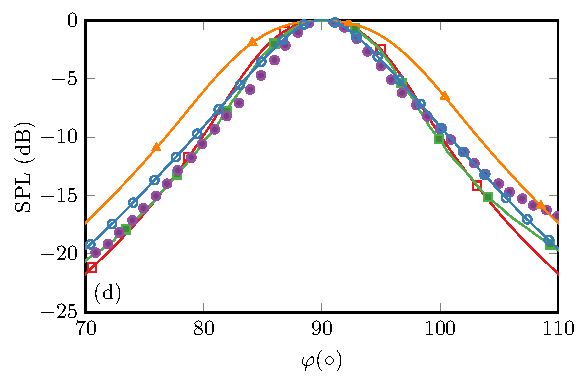
\includegraphics[width = \textwidth]{fig/Shi2015JasaFig4_4000Hz_Compare_v4_211014F.pdf}
    \end{subfigure}
    \caption{Audio SPL \revA{(dB re 20 $\mu$Pa)} generated by a conventional PAL with a uniform profile and a size of 0.08 m calculated using the convolution method and the cylindrical expansion at (a) 500 Hz, (b) 1 kHz, (c) 2 kHz, and (d) 4 kHz.
    Red hollow square, convolution model; blue hollow circle, cylindrical expansion at 4 m; orange triangle, cylindrical expansion in the far field; green solid square, convolution method from \cite{Shi2015ConvolutionModelComputing}; purple solid circle, measurement from \cite{Shi2015ConvolutionModelComputing}.}
    \label{fig:cwe_result_compare}
\end{figure}

The directivity of the audio sound beam in the far field can also be obtained using Eq.~(\ref{eq:conv}) of the convolution model, so the results calculated using this approach are presented in Fig.~\ref{fig:cwe_result_compare} for comparison. 
It can be seen in Fig.~\ref{fig:cwe_result_compare} that the SPL values calculated using the convolution model are slightly larger than the cylindrical expansion at a radius of 4 m for angles around $90^\circ$, and smaller at other angles. 
For example, in Fig.~\ref{fig:cwe_result_compare}(d) the SPL obtained at 4 m using the convolution model for a frequency of 4 kHz is 0.8 dB larger, and 1.6 dB smaller, than that obtained with a cylindrical expansion at $94.1^\circ$ and $102.1^\circ$, respectively. 
This difference becomes larger as the frequency decreases, indicating that the accuracy using the convolution model deteriorates at low frequencies.

The measured audio sound directivities at 4 kHz are available from \revA{Fig.~6} of \cite{Shi2015ConvolutionModelComputing}, and they are presented in Fig.~\ref{fig:cwe_result_compare}(d). 
The ultrasound directivities are required to obtain the audio sound directivity in the convolution model as shown in Eq.~(\ref{eq:conv}). 
They are predicted using Eqs.~(\ref{eq:cwe_potential}) and (\ref{eq:cwe_ultra_radial_far}), but obtained by measurement in \cite{Shi2015ConvolutionModelComputing}. 
Therefore, the results obtained using the convolution model in \cite{Shi2015ConvolutionModelComputing} can be different and they are also presented in Fig.~\ref{fig:cwe_result_compare}(d) for comparison. It can be seen in Fig.~\ref{fig:cwe_result_compare}(d) that the SPL values obtained with the cylindrical expansion at 4 m provides better agreement with measurement when compared to the convolution model, for angles larger than $85^\circ$. 
For example, the difference between measurement and the value obtained using the cylindrical expansion is only 0.5 dB at $94.8^\circ$, while it increases to 1.5 dB when compared to the convolution model. 


\subsubsection{Steerable PAL generating one beam}
\label{sec:cwe_one_beam}

The steerable PAL with a steering angle of $70^\circ$ used in Sec.~III.C of \cite{Shi2015ConvolutionModelComputing} is considered in this subsection. 
Figure~\ref{fig:cwe_results_one_beam} shows the audio sound fields at 4 kHz generated by a steerable PAL with a continuous or discrete profile, where the size of the phased array PAL is $2a = \SI{0.08}{m}$, and the size of the PAL unit is $a_0 = \SI{0.01}{m}$. 
Comparing Fig.~\ref{fig:cwe_results_one_beam}(a) to Fig.~\ref{fig:cwe_result_2d}(d), demonstrates the ability of a phased array PAL to steer the audio beam in a desired direction. When the velocity profile is discrete (which is usually limited by the size of real ultrasonic transducers), a side lobe would occur around $120^\circ$ as shown in Fig.~\ref{fig:cwe_results_one_beam}(b). 
This is known as the spatial aliasing phenomenon arising from the fact that the size of the PAL unit (0.01 m) is greater than the half of the wavelength of the ultrasound (0.0086 m at 40 kHz) \cite{Shi2011GratingLobeElimination}.

\begin{figure}[!htb]
    \centering
    \begin{subfigure}{0.49\textwidth}
        \centering
%        \includegraphics[width = \textwidth]{E:/Research/Pal2D2108/matlab/fig/Shi2015JasaFig6_FullField_v3_Case1_resize.jpg}
        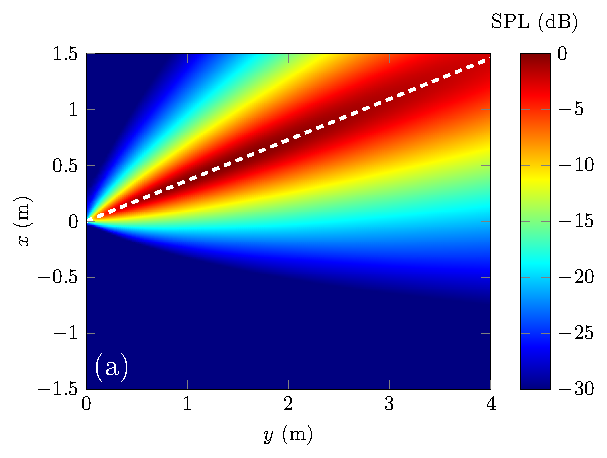
\includegraphics[width = \textwidth]{fig/Shi2015JasaFig6_FullField_v3_Case1.pdf}
    \end{subfigure}
    \begin{subfigure}{0.49\textwidth}
        \centering
        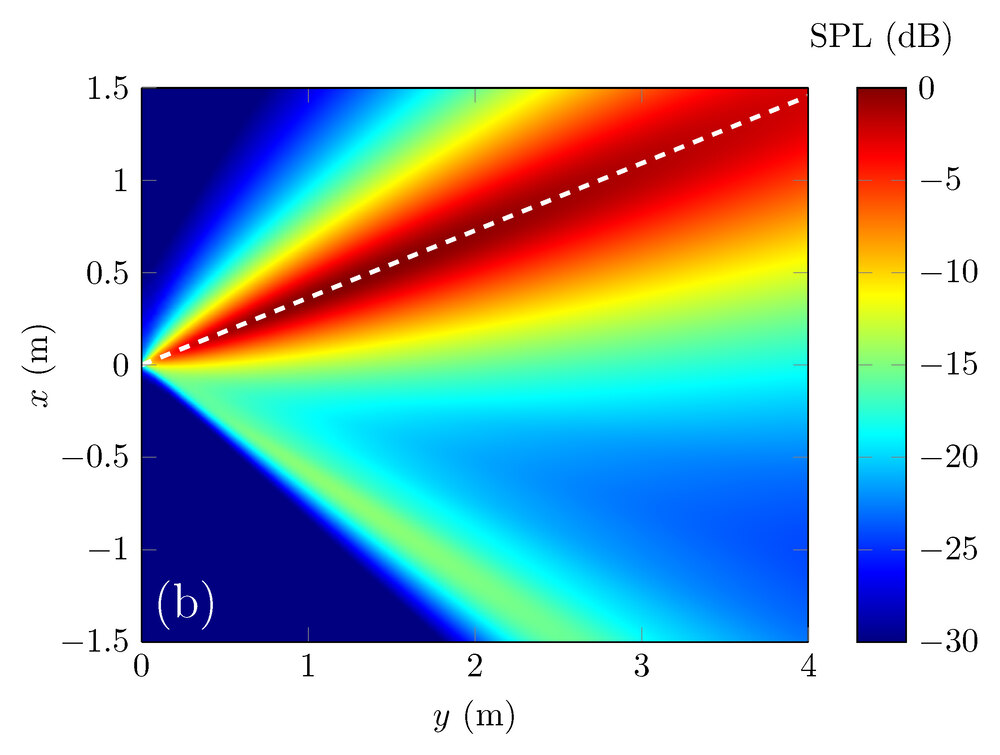
\includegraphics[width = \textwidth]{fig/Shi2015JasaFig6_FullField_v3_Case2_resize.jpg}
    \end{subfigure}
    \caption{Audio \revA{SPL (dB re 20 $\mu$Pa)} at 4 kHz generated by a steerable PAL with a steering angle of \ensuremath{70^\circ} (denoted by dashed lines), a size of 0.08 m, and a (a) continuous, or (b) discrete profile with a PAL unit size of 0.01 m. }
    \label{fig:cwe_results_one_beam}
\end{figure}

Figure~\ref{fig:cwe_results_one_beam_diff_angle} compares the audio SPL at different angles using the convolution model and the cylindrical expansion at a radial distance of 4 m. 
The measurement data and the results obtained using the convolution model and measured ultrasound directivities in \cite{Shi2015ConvolutionModelComputing} are also presented for comparison. 
It can be found both models can predict similar results around the main lobe at $70^\circ$. 
The side lobe is $115^\circ$ for the data in \cite{Shi2015ConvolutionModelComputing} while it is $120^\circ$ for the predictions in this section. 
The reason may arise from the measurement error, imperfect positioning of the phased array, and so on. 
The experimental result at the side lobe ($115^\circ$) in \cite{Shi2015ConvolutionModelComputing} is 3.1 dB below the prediction from the convolution model, which can be more accurately predicted by the cylindrical expansion as a decrement (3.0 dB) can be observed at the side lobe ($120^\circ$). 
It indicates the cylindrical expansion is more appropriate for the prediction of a steerable PAL with a discrete profile. 
Furthermore, the cylindrical expansion can predict the details of the sound field in the near field as shown in Fig.~\ref{fig:cwe_results_one_beam}.

\begin{figure}[!htb]
    \centering
    % \includegraphics[width = 0.5\textwidth]{E:/Research/Pal2D2108/matlab/fig/Shi2015JasaFig6_Directivity_Compare_v4.pdf}
    % \\
    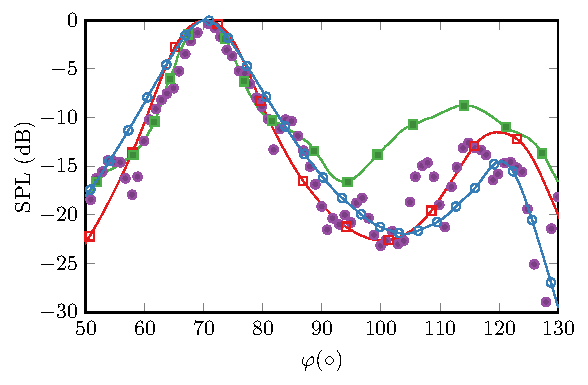
\includegraphics[width = 0.55\textwidth]{fig/Shi2015JasaFig6_Directivity_Compare_v4_211014G.pdf}
    \caption{Audio SPL \revA{(dB re 20 $\mu$Pa)} at 4 kHz at different angles generated by a steerable PAL with a steering angle of \ensuremath{70^\circ}, a size of 0.08 m, and a discrete profile with a PAL unit size of 0.01 m.
    Red hollow square, convolution model; blue hollow circle, cylindrical expansion at 4 m; green solid square, convolution model from \cite{Shi2015ConvolutionModelComputing}; purple solid circle, measurement from \cite{Shi2015ConvolutionModelComputing}.}
    \label{fig:cwe_results_one_beam_diff_angle}
\end{figure}

\subsubsection{Steerable PAL generating dual beams}
The generation of an unwanted side lobe when using a discrete velocity profile for a steerable PAL was shown in Sec.~\ref{sec:cwe_one_beam}. 
However, this effect can be utilized to generate dual audio beams, see \cite{Shi2011GratingLobeElimination} for more details. 
For example, Fig.~\ref{fig:cwe_results_dual_beam_2d} shows a 4 kHz dual audio beam at $70^\circ$ and $110^\circ$ using the parameters in Fig.~8 of \cite{Shi2015ConvolutionModelComputing}, and this was achieved by steering the ultrasound beams to $69^\circ$ and $71^\circ$ at 38 kHz and 42 kHz, respectively. 
The size of the phased array PAL is $2a = \SI{0.1}{m}$, the size of the PAL units is $a_0 = \SI{0.01}{m}$, their center separation is $a_1 = \SI{0.0125}{m}$, and the velocity profile is illustrated in Fig.~\ref{fig:cwe_velocity_profile}. 
The details of the audio sound in the near field shown in Fig.~\ref{fig:cwe_results_dual_beam_2d} demonstrates that this method can successfully generate dual beams with an acceptable acoustic contrast in the full field.

\begin{figure}[!htb]
    \centering
    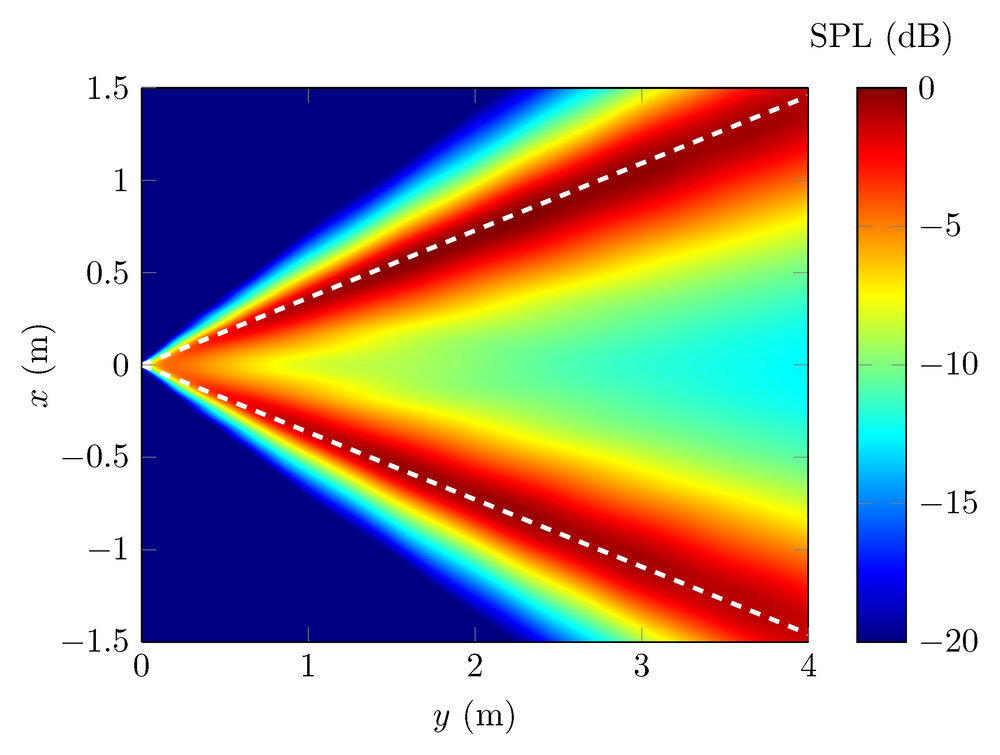
\includegraphics[width = 0.5\textwidth]{fig/Shi2015JasaFig8_FullField_v3_resize.jpg}
    \caption{Audio \revA{SPL (dB re 20 $\mu$Pa)} at 4 kHz generated by a steerable PAL generating dual beams at \ensuremath{70^\circ} and \ensuremath{110^\circ} (denoted by dashed lines), where the size of the phased array PAL is 0.1 m, the size of PAL units is 0.01 m, and their center separation is 0.0125 m.}
    \label{fig:cwe_results_dual_beam_2d}
\end{figure}

The audio SPL at different angles, obtained using the proposed cylindrical expansion and the convolution model is compared in Fig.~\ref{fig:cwe_results_dual_beam}. 
The measurement data and the results obtained using the convolution model and ultrasound directivities in \cite{Shi2015ConvolutionModelComputing} are also presented. 
As shown in Fig.~\ref{fig:cwe_results_dual_beam}, it is clear the cylindrical expansion provides a much better agreement with the measurement data. 
At the angles between two lobes the SPL values obtained using the convolution model are lower than those found using the cylindrical expansion. 
The difference between the two is a maximum of 5.8 dB at $90^\circ$. 
The nonlinear interactions between ultrasonic waves in the near field becomes more complex in this case when compared to a conventional PAL with a uniform excitation. 
These interactions cannot be captured in the convolution model because only the far field directivity for ultrasound is used. The prediction accuracy is, therefore, deteriorated significantly in this case. 
However, no simplifications for ultrasound are made in the cylindrical expansion, so it provides a more accurate solution. 

\begin{figure}[!htb]
    \centering
    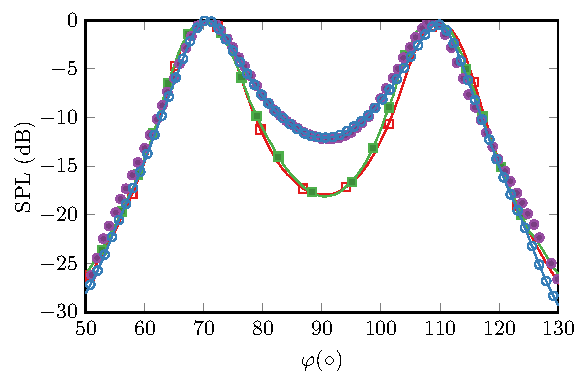
\includegraphics[width = 0.55\textwidth]{fig/Shi2015JasaFig8_Directivity_Compare_v4_211014H.pdf}
    \caption{Audio \revA{SPL (dB re 20 $\mu$Pa)} at 4 kHz at different angles generated by a steerable PAL generating dual beams at $70^\circ$ and $110^\circ$, where the size of the phased array PAL is 0.1 m, the size of PAL units is 0.01 m, and their center separation is 0.0125 m.
    Red hollow square, convolution model; blue hollow circle, cylindrical expansion at 4 m; green solid square, convolution model from \cite{Shi2015ConvolutionModelComputing}; Purple solid circle, measurement from \cite{Shi2015ConvolutionModelComputing}.}
    \label{fig:cwe_results_dual_beam}
\end{figure}


\section{Summary}
A SWE is derived for the sound radiation from a baffled circular source in Sec.~\ref{Section41}.
A closed-form for the calculation of the radial component is proposed based on the recurrence relation of spherical Bessel functions. 
Unlike the existing GHF method, the Gauss-Legendre quadrature, and the infinite Bessel expansion, the proposed expression can be calculated exactly with finite terms in the whole frequency range. 
In the proposed expression, the spherical coordinates of the field point and the disk radius are uncoupled, which is convenient for obtaining derivatives and integrals with respect to these parameters. 
The proposed method can also be extended to other scenarios, such as the radiation from a baffled circular piston with axisymmetric velocity profiles, a resilient disk in free space, and a baffled rotating source \cite{Zhong2020SphericalExpansionCalculating}. 

Section \ref{sec:swe_pal} extends the SWE for the radiation of a baffled circular PAL.
The key step is to express the Green's function of a point monopole in free field by a series consisting of trigonometric, Legendre, and spherical Bessel functions, so that the five-fold integral in the expression of audio sounds generated by a PAL can be simplified to three-fold summations by using the orthogonal properties of the trigonometric and Legendre functions. 
The proposed expression has the uncoupled angular component determined by Legendre polynomials and the radial one which is a rapidly converged integral involving spherical Bessel functions which converges rapidly. 
Unlike the widely used GBE method, the proposed expansion avoids the additional Fresnel approximation and can be calculated efficiently. In the numerical simulations, the GBE method is at least 15 times slower than the proposed method and shows poor convergence in the near field while the proposed method is computationally efficient in \revA{both the near and far fields}. 

In Sec.~\ref{sec:cwe_source}, a cylindrical expansion for the radiation from infinitely long strips was reviewed. 
The cylindrical expansion was then extended in Sec.~\ref{sec:cwe_pal} for the audio sound generated by a PAL after adopting the phased array technique based on a quasilinear solution of the Westervelt equation. 
The expansion is a series of twofold summations with uncoupled angular and radial components in the cylindrical coordinate system. The angular component is determined by the trigonometric functions, and the radial one is an integral containing the Bessel functions and an arbitrary excitation velocity profile. The proposed expansion converges much faster than the direct numerical integration of the quasilinear solution.

The numerical results are presented for several steerable PALs and compared to predictions obtained using the convolution model. A comparison with measurements reported by Shi and Kajikawa, in Figs.~\ref{fig:cwe_result_compare}, \ref{fig:cwe_results_one_beam_diff_angle}, and \ref{fig:cwe_results_dual_beam} demonstrates that the proposed cylindrical expansion provides better agreement with measurement when compared to the convolution model. This is because the complex nonlinear interactions of the ultrasound waves in the near field are correctly captured by the cylindrical expansion. In addition, the proposed cylindrical expansion in Eqs.~(\ref{eq:cwe_audio}) and (\ref{eq:cwe_audio_radial_component}) can predict the near audio sound field as shown in Sec.~\ref{sec:cwe_results}, whereas it is not applicable for the convolution model in Eq.~(\ref{eq:conv}). 

The cylindrical expansion requires that the radiation surface of the PAL array is infinitely long in one dimension. 
This requirement is easy to satisfy because the ultrasonic wavelength is usually much smaller than an ordinary PAL. However, this is not always the case for the audio sound and so prediction accuracy at low audio frequencies may deteriorate when using the cylindrical expansion and this remains to be addressed. Nevertheless, the proposed cylindrical expansion is shown to provide a computationally efficient approach to modelling a PAL after adopting the phased array technique.

